% !TEX program = xelatex
% 电工电子技术 · 第五章 集成运算放大器 · 精讲讲义（lecture-deepdive 规范）
\documentclass[11pt]{ctexart}
%=====================================================================
% theme-violet.tex —— 讲义精讲 · 紫花主题
% 用法：\documentclass[11pt]{ctexart}
%       \input{assets/theme-violet}
%       \begin{document} ... \end{document}
% 只用 ctexart 自带能力 + xcolor/enumitem/fancyhdr/pifont/amsmath，
% 不依赖 tikz/tcolorbox，保证 MiKTeX 可直接编译。
%=====================================================================

\usepackage[a4paper,left=2.0cm,right=2.0cm,top=2.1cm,bottom=2.3cm,%
            headsep=12pt,footskip=22pt]{geometry}
\usepackage{amsmath,amssymb}
\usepackage{xcolor}
\usepackage{array}
\usepackage{enumitem}
\usepackage{pifont}
\usepackage{fancyhdr}
\usepackage[hidelinks]{hyperref}

%---------------------------------------------------------------- 配色
\definecolor{violet}{RGB}{107,78,143}      % 主色：紫
\definecolor{violetdeep}{RGB}{63,44,92}    % 深紫：标题/强调
\definecolor{petal}{RGB}{183,159,208}      % 花瓣：装饰线、花饰
\definecolor{bandviolet}{RGB}{247,243,251} % 浅紫底：档案/提示框
\definecolor{bandcream}{RGB}{252,249,242}  % 米白底：易错/注意框
\definecolor{rulepurple}{RGB}{217,207,230} % 分隔线
\definecolor{inkgray}{RGB}{92,96,110}      % 次要文字

%---------------------------------------------------------------- 字体
% 有 Noto CJK 用 Noto，没有就退回 ctex 默认（Windows 下为宋体/黑体）
\IfFontExistsTF{Noto Serif CJK SC}{\setCJKmainfont{Noto Serif CJK SC}}{}
\IfFontExistsTF{Noto Sans CJK SC}{\setCJKsansfont{Noto Sans CJK SC}}{}

%---------------------------------------------------------------- 版式
\setlist{nosep,leftmargin=1.9em}
\linespread{1.28}
\setlength{\parskip}{3.5pt}
\setlength{\parindent}{0pt}
\setlength{\tabcolsep}{5pt}
\renewcommand{\arraystretch}{1.28}

%---------------------------------------------------------------- 花饰
% \ding{95} = 五瓣小花，\ding{96} = 星形花；都来自 pifont，必定存在
\newcommand{\orn}{\textcolor{petal}{\ding{95}}}          % 行内小标
\newcommand{\ornstar}{\textcolor{petal}{\ding{96}}}      % 星形花
\newcommand{\flowerrule}{%                                % 居中花饰分隔线
  \par\vspace{7pt}%
  \noindent\makebox[\linewidth]{\color{petal}%
    \rule{0.20\linewidth}{0.6pt}\hspace{8pt}{\small\ding{95}}\hspace{4pt}%
    \raisebox{1.1pt}{\tiny\ding{95}}\hspace{4pt}{\small\ding{95}}\hspace{8pt}%
    \rule{0.20\linewidth}{0.6pt}}%
  \par\vspace{7pt}}

%---------------------------------------------------------------- 标题与节头
\newcommand{\doctitle}[3]{%   #1 主标题  #2 副标题  #3 元信息（可用 \\ 分行）
  \begin{center}
    {\color{petal}\small \orn\enspace #2\enspace \ornstar}\\[7pt]
    {\LARGE\bfseries\color{violetdeep} #1}\\[10pt]
    {\color{petal}\rule{0.55\linewidth}{1pt}}\\[4pt]
    {\small\color{inkgray} #3}
  \end{center}\vspace{2pt}}

\newcommand{\hdr}[2]{%   #1 章节号（如 §0）  #2 标题
  \par\vspace{12pt}%
  \noindent\colorbox{violetdeep}{\color{white}\bfseries\small\;#1\;}\hspace{7pt}%
  {\color{violetdeep}\large\bfseries #2}\par\nobreak
  \vspace{3pt}{\color{petal}\hrule height 1.2pt}\vspace{6pt}}

\newcommand{\subhdr}[1]{%
  \par\vspace{6pt}%
  \noindent{\color{violet}\bfseries #1}\par\vspace{1pt}}

%---------------------------------------------------------------- 提示框
\newcommand{\callout}[1]{% 浅紫底：讲义档案、读法说明
  \par\medskip\noindent
  \fcolorbox{rulepurple}{bandviolet}{\parbox{\dimexpr\linewidth-2\fboxsep-2\fboxrule}{\vspace{2pt}#1\vspace{2pt}}}%
  \par\medskip}

\newcommand{\warnbox}[1]{% 米白底：易错、边界条件
  \par\medskip\noindent
  \fcolorbox{rulepurple}{bandcream}{\parbox{\dimexpr\linewidth-2\fboxsep-2\fboxrule}{\vspace{2pt}#1\vspace{2pt}}}%
  \par\medskip}

\newcommand{\gapitem}[2]{% #1 缺口类型（紫） #2 内容
  \par\vspace{2pt}\noindent
  \hangindent=1.4em\hangafter=1
  {\color{petal}\small\ding{96}}\enspace{\bfseries\color{violetdeep}#1}\enspace #2\par}

% 前提旁注：只放在「需要理解的那一步」后面，给陈述 + 本题代入，不重证。
\newcommand{\aside}[1]{%
  \par\vspace{1pt}\noindent
  \hangindent=1.6em\hangafter=1
  {\small\color{inkgray}%
    \hspace*{0.6em}{\color{petal}$\triangleright$}\hspace{2pt}#1}%
  \par\vspace{2pt}}

%---------------------------------------------------------------- 表格
% 本机 MiKTeX 的 colortbl 与 array 版本不匹配（\rowcolor 会报错），
% 故表格统一用「上粗紫线 + 表头 + 中细线」的三线式，不依赖 colortbl。
\newcommand{\tabtop}{\par\vspace{3pt}{\color{violet}\hrule height 1.2pt}\vspace{1pt}}
\newcommand{\tabmid}{\par\vspace{1pt}{\color{petal}\hrule height 0.5pt}\vspace{1pt}}
\newcommand{\tabbot}{\par\vspace{3pt}{\color{rulepurple}\hrule height 0.5pt}\vspace{8pt}}
\newcommand{\thead}[1]{{\bfseries\color{violetdeep}#1}}

%---------------------------------------------------------------- 页眉页脚
\pagestyle{fancy}
\fancyhf{}
\renewcommand{\headrulewidth}{0.4pt}
\renewcommand{\headrule}{\hbox to\headwidth{\color{rulepurple}\leaders\hrule height \headrulewidth\hfill}}
\fancyhead[L]{\small\color{inkgray}\songti \doctag}
\fancyhead[R]{\small\color{inkgray}\songti \coursetag}
\fancyfoot[C]{\small\color{inkgray}\orn\enspace{\color{violet}\thepage}\enspace\orn}

% 每篇讲义在导言区设这两个值
\newcommand{\doctag}{}
\newcommand{\coursetag}{}
\newcommand{\settags}[2]{\renewcommand{\doctag}{#1}\renewcommand{\coursetag}{#2}}

%---------------------------------------------------------------- 数学记号
\newcommand{\vect}[1]{\boldsymbol{#1}}
\newcommand{\dd}{\,\mathrm{d}}
\newcommand{\ddx}{\frac{\mathrm{d}}{\mathrm{d}x}}
\addtolength{\jot}{2pt}



\usepackage{booktabs}
\usepackage{tikz}
\usetikzlibrary{arrows.meta,calc}
% 可跨页的提示框（主题里的 \callout / \warnbox 是单参数命令、内部用 parbox，
% 长段落会溢出一页；这里改用 tcolorbox 的可断页版本，配色沿用主题）
\usepackage[most]{tcolorbox}
\newtcolorbox{cbox}{enhanced,breakable,colback=bandviolet,colframe=rulepurple,
  boxrule=0.5pt,arc=1.5pt,left=6pt,right=6pt,top=4pt,bottom=4pt,
  before skip=5pt,after skip=5pt}
\newtcolorbox{wbx}{enhanced,breakable,colback=bandcream,colframe=rulepurple,
  boxrule=0.5pt,arc=1.5pt,left=6pt,right=6pt,top=4pt,bottom=4pt,
  before skip=5pt,after skip=5pt}
\settags{Ch5-1 · 集成运算放大器 · 精讲（20261029 版）}{电工电子技术}
\setlength{\emergencystretch}{3em}
\tracinglostchars=2

%=============================================================
% 比较器小电路：#1 反相端电压 #2 同相端电压 #3 电源标号 #4 答案 #5 输出端二极管
%   #5 = 0 不接；1 = 左普通管朝上 + 右 LED 朝下；2 = 左 LED 朝上 + 右普通管朝下
%=============================================================
\newcommand{\cmpfig}[5]{%
\begin{tikzpicture}[line width=0.7pt,scale=0.80,font=\footnotesize,
    every node/.append style={inner sep=1.2pt}]
  \draw (0,0) rectangle (1.70,1.60);
  \node[anchor=west] at (0.10,1.20) {$-$};
  \node[anchor=west] at (0.10,0.40) {$+$};
  \fill (1.02,1.13)--(1.16,1.21)--(1.02,1.29)--cycle;
  \node[anchor=west] at (1.24,1.21) {$\infty$};
  \draw (-1.25,1.20)--(0,1.20);
  \node[anchor=east] at (-1.32,1.20) {#1};
  \draw (-1.25,0.40)--(0,0.40);
  \node[anchor=east] at (-1.32,0.40) {#2};
  \draw (0.85,1.60)--(0.85,2.00);
  \node[circle,draw,fill=white,inner sep=1.1pt] at (0.85,2.00) {};
  \node[anchor=west] at (1.02,2.00) {#3};
  \draw (1.70,0.80)--(2.55,0.80);
  \node[circle,draw,fill=white,inner sep=1.1pt] at (2.55,0.80) {};
  \node[anchor=west] at (2.68,0.80) {$u_{\mathrm{O}}$};
  \node[fill=bandviolet,draw=rulepurple,inner sep=2.4pt,anchor=west] at (3.60,0.80) {#4};
  \ifnum#5>0
    \draw (2.00,0.80)--(2.00,-0.05);
    \draw (2.55,0.80)--(2.55,-0.05);
    \draw (1.80,-0.80)--(2.75,-0.80);
    % ---- 左侧管
    \ifnum#5=1
      % 普通二极管，朝上（阳极在下的地，阴极在上的输出）⇒ 输出为负时导通
      \draw (1.87,-0.05)--(2.13,-0.05);
      \draw (1.87,-0.40)--(2.13,-0.40);
      \draw (1.87,-0.40)--(2.00,-0.05)--(2.13,-0.40);
      \draw (2.00,-0.40)--(2.00,-0.80);
      \node[anchor=east] at (1.74,-0.86) {\scriptsize D};
    \else
      % LED，朝上
      \draw (1.87,-0.05)--(2.13,-0.05);
      \draw (1.87,-0.40)--(2.13,-0.40);
      \fill (1.88,-0.40)--(2.12,-0.40)--(2.00,-0.08)--cycle;
      \draw (2.00,-0.40)--(2.00,-0.80);
      \node[anchor=east] at (1.74,-0.86) {\scriptsize LED};
    \fi
    % ---- 右侧管
    \ifnum#5=1
      % LED，朝下（阳极在上的输出）⇒ 输出为正时导通
      \draw (2.42,-0.05)--(2.68,-0.05);
      \draw (2.42,-0.40)--(2.68,-0.40);
      \fill (2.43,-0.05)--(2.67,-0.05)--(2.55,-0.37)--cycle;
      \draw (2.55,-0.40)--(2.55,-0.80);
      \node[anchor=west] at (2.81,-0.86) {\scriptsize LED};
    \else
      % 普通管，朝下
      \draw (2.42,-0.05)--(2.68,-0.05);
      \draw (2.42,-0.40)--(2.68,-0.40);
      \draw (2.42,-0.05)--(2.55,-0.40)--(2.68,-0.05);
      \draw (2.55,-0.40)--(2.55,-0.80);
      \node[anchor=west] at (2.81,-0.86) {\scriptsize D};
    \fi
  \fi
\end{tikzpicture}}


%=============================================================
% 家族电路宏：课件 p29/p30/p32/p35 的示范电路与 p36--p43 的 E1--E8
% 全部属于同一拓扑家族，只差三个开关：
%   #2 输入端（1=反相端在上，2=同相端在下）
%   #3 反馈端（1=反相端，2=同相端）
%   #4 取样点（1=输出端 ⇒ VF，2=R_L 与 R 之间 ⇒ CF）
%   #5/#6 输入电阻与偏置电阻的标注名；#7 几何缩放
%   #1（可选）非空 ⇒ 叠印瞬时极性法的三个 ⊕ 标记
%=============================================================
\newcommand{\famcirc}[7][]{%
\begin{tikzpicture}[line width=0.7pt,>=Latex,scale=#7,font=\scriptsize,
    every node/.append style={inner sep=1.0pt}]
  \def\yA{1.65}\def\yB{0.55}\def\xL{3.55}\def\xF{4.95}
  \def\yS{1.10}
  % ---------- 放大器
  \draw (0,0) rectangle (2.30,2.20);
  \node[anchor=west] at (0.10,\yA) {$-$};
  \node[anchor=west] at (0.10,\yB) {$+$};
  \node at (1.42,1.10) {$A_{\mathrm{o}}$};
  \fill (1.92,1.71)--(2.10,1.80)--(1.92,1.89)--cycle;
  % ---------- 输出与负载
  \draw (2.30,1.10)--(\xL,1.10);
  \draw (\xL,1.10)--(\xL,0.92);
  \draw[fill=white] (\xL-0.12,0.92) rectangle (\xL+0.12,0.46);
  \node[anchor=east] at (\xL-0.20,0.69) {$R_{\mathrm{L}}$};
  \node at (\xL+0.16,0.90) {$+$};
  \node[anchor=west] at (\xL+0.46,0.69) {\color{violetdeep}$u_{\mathrm{O}}$};
  \node at (\xL+0.16,0.48) {$-$};
  \ifnum#4=1
    \draw (\xL,0.46)--(\xL,0.14);
    \draw (\xL-0.20,0.14)--(\xL+0.20,0.14);
    \draw (\xL-0.13,0.03)--(\xL+0.13,0.03);
    \draw (\xL-0.05,-0.08)--(\xL+0.05,-0.08);
  \else
    \def\yS{0.24}
    \draw (\xL,0.46)--(\xL,0.24);
    \draw[fill=white] (\xL-0.12,-0.06) rectangle (\xL+0.12,-0.52);
    \draw (\xL,0.24)--(\xL,-0.06);
    \draw (\xL,-0.52)--(\xL,-0.80);
    \draw (\xL-0.20,-0.80)--(\xL+0.20,-0.80);
    \draw (\xL-0.13,-0.91)--(\xL+0.13,-0.91);
    \draw (\xL-0.05,-1.02)--(\xL+0.05,-1.02);
    \node[anchor=east] at (\xL-0.20,-0.29) {$R$};
  \fi
  % ---------- 输入与偏置
  \ifnum#2=1 \def\yI{\yA}\def\yG{\yB}\else \def\yI{\yB}\def\yG{\yA}\fi
  \def\xn{-3.05}\def\xr{-2.35}\def\xrR{-1.55}
  \draw (\xn,\yI) circle (0.055);
  \draw (\xn,\yI)--(\xr,\yI);
  \draw[fill=white] (\xr,\yI-0.13) rectangle (\xrR,\yI+0.13);
  \draw (\xrR,\yI)--(0,\yI);
  \node[anchor=east] at (\xn-0.10,\yI) {$u_{\mathrm{I}}$};
  \node[anchor=north] at ({(\xr+\xrR)/2},\yI-0.17) {$#5$};
  \draw (0,\yG)--(\xrR,\yG);
  \draw[fill=white] (\xr,\yG-0.13) rectangle (\xrR,\yG+0.13);
  \draw (\xr,\yG)--(\xn+0.24,\yG);
  \draw (\xn+0.24,\yG)--(\xn+0.24,\yG-0.13);
  \draw (\xn+0.01,\yG-0.13)--(\xn+0.47,\yG-0.13);
  \draw (\xn+0.09,\yG-0.24)--(\xn+0.39,\yG-0.24);
  \draw (\xn+0.17,\yG-0.35)--(\xn+0.31,\yG-0.35);
  \node[anchor=north] at ({(\xr+\xrR)/2},\yG-0.17) {$#6$};
  % ---------- 反馈
  \ifnum#3=1 \def\yF{\yA}\def\yR{2.86}\else \def\yF{\yB}\def\yR{-1.66}\fi
  \def\xf{-0.60}
  \draw (\xf,\yF)--(\xf,\yR);
  \draw (\xf,\yR)--(-0.35,\yR);
  \draw[fill=white] (-0.35,\yR-0.13) rectangle (0.45,\yR+0.13);
  \draw (0.45,\yR)--(\xF,\yR);
  \ifnum#3=1
    \node[anchor=north] at (0.05,\yR-0.18) {$R_{\mathrm{F}}$};
  \else
    \node[anchor=south] at (0.05,\yR+0.18) {$R_{\mathrm{F}}$};
  \fi
  \draw (\xF,\yR)--(\xF,\yS);
  \draw (\xF,\yS)--(\xL,\yS);
  \fill (\xL,\yS) circle (0.055);
  \fill (\xf,\yF) circle (0.045);
  % ---------- 可选标注：#1 = pol ⇒ 瞬时极性法的三个 ⊕；#1 = q ⇒ 标出 Q 点
  \def\polmark{#1}\def\cmppol{pol}\def\cmpq{q}%
  \ifx\polmark\cmppol
    \node[circle,draw,thick,fill=white,inner sep=1.6pt] at (\xn+0.30,\yI) {$+$};
    \node[circle,draw,thick,fill=white,inner sep=1.6pt] at (\xL-0.70,1.10) {$+$};
    \node[circle,draw,thick,fill=white,inner sep=1.6pt] at (\xf,\yF) {$+$};
  \fi
  \ifx\polmark\cmpq
    \ifnum#3=1
      \node at (\xf-0.04,\yF+0.30) {\textbf{Q}};
    \else
      \node at (\xf-0.04,\yF-0.32) {\textbf{Q}};
    \fi
  \fi
\end{tikzpicture}}







\begin{document}
\doctitle{第五章　集成运算放大器}
{从一只「增益无穷大的差动放大器」，到「负反馈怎么把增益变成控制力」}
{依据：\texttt{Chapter Five-1-2026中白上传(1).pdf}（p1--p50，共 50 页）\ \textperiodcentered\ 2026-10-29}

\begin{cbox}
\textbf{这份讲义怎么用}：§0 是课件坐标，先把「这 50 页讲了什么、缺了哪一节」对齐；
§1--§3 讲运放本身（是什么、输出随净输入怎么变、开环时它只能当比较器）；
§4--§5 是本章的主体，讲反馈的概念、三条判据，并把课件 p36--p43 的八道判定题（E1--E8）
\textbf{一题一块}判完；§6 讲负反馈换来什么；§7 落到「虚短虚断」并立刻用它解两个电路。

每个结论后面都带课件页码（写成 \texttt{[C5-1 p13]} 这种形式），可以回原页核对；
凡课件没写而本讲义补的，都标「[补]」或在 §10 的缺口清单里逐条点名。
\textbf{八道判定题不必背答案}——§5.5 末尾用一张 $2\times2\times2$ 的表把八题的规律摊开，
记住三条判据各看一处，比记八个答案管用。
\end{cbox}

\subhdr{本讲义结构}

\begin{center}
\small
\begin{tabular}{@{}p{1.4cm}p{13.4cm}@{}}
\toprule
\thead{节} & \thead{内容}
\\
\midrule
§0 & 课件坐标：50 页的分段表、缺失的 5.4、记号统一表
\\
§1 & 5.1 集成运放：IC 与集成规模、理想三条件、三级结构、741 引脚、等效电路（图 1-1、1-2）
\\
§2 & 5.2 电压传输特性：三个区、线性区只有 $12\ \mu\mathrm{V}$ 宽、$A_{\mathrm{o}}$ 越大越陡（图 2-1）
\\
§3 & 5.3 比较器：为什么只有两个值、四道例题全解（图 3-1）
\\
§4 & 5.5.1 反馈的概念：定义与三张接法图、开环/闭环、框图三系数（图 4-1、4-2）
\\
§5 & 5.5.2 反馈的类型：三条判据（正负 / 电压电流 / 串并）+ E1--E8 一题一块（图 5-1--5-11）
\\
§6 & 5.5.3 负反馈的影响：$A_{\mathrm{F}}$ 与 $A_{\mathrm{o}}$ 的关系、五样好处（图 6-1、6-2）
\\
§7 & 5.6 虚短与虚断：三条假设、成立的两条条件、两道解题示范（图 7-1--7-3）
\\
§8 & 公式卡四张 + 拿到电路后的四步用法
\\
§9 & 易错点 8 条，每条指回某一步
\\
§10 & 缺口清单 15 条，逐条给页码与原文短语
\\
§11 & 三句话总结
\\
§12 & 与课件的页码对照表（p1--p50 逐段）
\\
\bottomrule
\end{tabular}
\end{center}

\clearpage

%=============================================================
\hdr{§0}{课件坐标：这 50 页讲了什么，缺了哪一节}

\subhdr{先认课件：Chapter Five-1 是第五章的第一份}

课件文件名是 \texttt{Chapter Five-1-2026中白上传.pdf}，共 50 页，页眉写
\textbf{Circuits and Electronics}、正文节号从 \textbf{5.1 Introduction to Integrated Op Amp}
到 \textbf{5.6 Important conclusion of Op-amp}，p1 大标题是 \textbf{Chapter 5 Integrated Operational Amplifier}，
落款 Dalian University of Technology。所以它\textbf{确实是第 5 章}（集成运算放大器）的第一份。

本讲义所有坐标写成 \texttt{[C5-1 p13]} 这种形式：\texttt{C5-1} 指这份文件，
\texttt{p} 后面的数字指该 PDF 的\textbf{物理页码}（右下角那个数字，p1 是封面，没有前置页）。
凡是回指课件的结论，都带这样一枚坐标；凡是本讲义自己补的，都标明「补」。

\subhdr{这 50 页的分段}

\begin{center}
\small
\begin{tabular}{@{}p{2.0cm}p{3.5cm}p{7.3cm}p{2.4cm}@{}}
\toprule
\thead{页码} & \thead{页眉节号} & \thead{内容} & \thead{本讲义落点}
\\
\midrule
p1 & 5.1 & 封面：本章标题与 5.1 节名 & ---
\\
p2 & 5.1 & IC 是什么、能干什么 & §1.1
\\
p3--p6 & 5.1 & 集成规模四档：SSI / MSI / LSI / VLSI & §1.2
\\
p7--p8 & 5.1 & 理想放大器的三条条件 & §1.3
\\
p9 & 5.1 & 运放内部三级结构 & §1.4
\\
p10 & 5.1 & 理想参数与实际参数四个对照 & §1.5
\\
p11 & 5.1 & 符号与每个标注的含义 & §1.6
\\
p12 & 5.1 & 741 引脚配置与双电源 & §1.7
\\
p13 & 5.1 & 等效电路（差动放大的模型） & §1.8
\\
p14 & 5.1 & 一道题：$u_{\mathrm{D}}{=}3\ \mathrm{mV}$、$A_{\mathrm{o}}{=}10^{6}$，求输出 & §1.9
\\
p15--p20 & 5.2 & 电压传输特性：定义与三段 & §2
\\
p21--p22 & 5.3 & 比较器原理与四道例题 & §3
\\
p23--p26 & 5.5.1 & 反馈的定义、开环/闭环、框图三系数 & §4
\\
p27 & 5.5.2 & 反馈的三个分类维度 & §5.1
\\
p28--p30 & 5.5.2 & 判据一：正/负（瞬时极性法） & §5.2
\\
p31--p32 & 5.5.2 & 判据二：电压/电流（输出短路法） & §5.3
\\
p33--p35 & 5.5.2 & 判据三：串联/并联（Q 点接地法） & §5.4
\\
p36--p43 & 5.5.2 & 八道判定题 E1--E8 & §5.5
\\
p44--p48 & 5.5.3 & 负反馈的影响：增益关系与四样好处 & §6
\\
p49--p50 & 5.6 & 理想特性与深度负反馈的三条假设 & §7
\\
\bottomrule
\end{tabular}
\end{center}

\subhdr{一处必须点名的拼接：没有 5.4}

p22 的页眉是 \textbf{5.3 Comparator circuit}，p23 的页眉直接变成 \textbf{5.5 Basic concept of feedback}，
中间\textbf{没有 5.4 这一节}。这不是排版小错：按课件自己的编号体系，5.1--5.3 讲的是「运放是什么、
它的输出随净输入怎么变、开环时它只能当比较器」，5.5 起才讲「反馈怎么把输出送回输入端」，
两者之间缺的正是\textbf{「把理想特性用到线性电路上需要什么前提」}这一步。

本讲义不猜 5.4 的标题是什么，只补它该提供的桥：§7 把「虚短、虚断」作为\textbf{深度负反馈的结论}
正式推出（而不是当成口诀背），§7.4 立刻用这两条假设解两个最基本的有源电路，让读者看到
「有这两条就能算」而不是「背下来考试用」。

\subhdr{记号：先说清楚，后文不再回头}

课件混用 $A_{\mathrm{O}}$、$A_{\mathrm{o}}$、$A_0$ 三种写法表示开环增益，混用 $-U_{\mathrm{O(sat)}}$
与 $-U_{\mathrm{OM}}$ 表示负向饱和电压。本讲义统一如下：

\begin{center}
\small
\begin{tabular}{@{}p{3.4cm}p{12.2cm}@{}}
\toprule
\thead{记号} & \thead{含义（课件里的对应写法）}
\\
\midrule
$u_-$、$u_+$ & 反相端、同相端对地的电压（课件 $u_-$、$u_+$）
\\
$u_{\mathrm{D}}$ & 净输入（net input），$u_{\mathrm{D}}=u_+-u_-$（课件 $u_{\mathrm{D}}$、$u_D$）
\\
$u_{\mathrm{O}}$ & 输出电压（课件 $u_{\mathrm{O}}$、$u_{\mathrm{o}}$、$u_o$）
\\
$A_{\mathrm{o}}$ & 开环电压增益（课件 $A_{\mathrm{o}}$、$A_{\mathrm{O}}$、$A_0$、$A_o$）
\\
$A_{\mathrm{F}}$ & 闭环电压增益，$A_{\mathrm{F}}=x_{\mathrm{O}}/x_{\mathrm{I}}$（课件 $A_{\mathrm{F}}$）
\\
$F$ & 反馈系数，$F=x_{\mathrm{F}}/x_{\mathrm{O}}$（课件 $F$）
\\
$x_{\mathrm{I}}$、$x_{\mathrm{D}}$、$x_{\mathrm{O}}$、$x_{\mathrm{F}}$ & 输入、净输入、输出、反馈信号（框图里的通用量，可以是电压也可以是电流）
\\
$U_{\mathrm{OM}}$ & 输出饱和电压的幅值，$u_{\mathrm{O}}=+U_{\mathrm{OM}}$ 或 $-U_{\mathrm{OM}}$（课件 $+U_{\mathrm{O(sat)}}$、$+U_{\mathrm{OM(sat)}}$）
\\
$U_{\mathrm{CC}}$、$U_{\mathrm{EE}}$ & 正电源、负电源（课件 $+U_{\mathrm{CC}}$、$-U_{\mathrm{EE}}$）
\\
$r_{\mathrm{i}}$、$r_{\mathrm{o}}$ & 输入电阻、输出电阻
\\
CMRR & 共模抑制比（Common Mode Rejection Ratio）
\\
$R_1$、$R_2$、$R_{\mathrm{F}}$、$R_{\mathrm{L}}$、$R$ & 课件 E1--E8 的五个电阻：输入端串联电阻、另一端对地电阻、反馈电阻、负载、电流取样电阻
\\
NF / PF & 负反馈 / 正反馈（Negative / Positive Feedback）
\\
VF / CF & 电压反馈 / 电流反馈（Voltage / Current Feedback）
\\
SF / PF$'$ & 串联反馈 / 并联反馈（Series / Parallel Feedback）
\\
\bottomrule
\end{tabular}
\end{center}

\aside{注意两个撞车的缩写：课件里 \textbf{PF} 同时用来表示「正反馈」和「并联反馈」。
本讲义一律写全：正反馈写 \textbf{正反馈}，并联反馈写 \textbf{并联}，不再用 PF 这个缩写。}

\subhdr{全章只有一条主线}

\callout{\textbf{一句话主线}：运放的开环增益\textbf{无穷大}，所以只要两个输入端差一丁点，
输出就顶到电源——这让它\textbf{开环只能当比较器}（§3）；要让它在线性区里精确工作，
只能用\textbf{负反馈}把两个输入端「摁」在一起（§4--§7），代价是增益变小，换来的是
\textbf{增益稳定、频带变宽、失真变小、阻抗可控}（§6），以及两个可以当公式用的结论——
\textbf{虚短} $u_+=u_-$ 与\textbf{虚断} $i_+=i_-=0$（§7）。

后面每一节都只是这句话的一段展开。读的时候随时问自己：这一页在讲「无穷大」的哪个后果？}

%=============================================================
\hdr{§1}{5.1 集成运放：从一块硅片到一只符号}

\subhdr{IC 是什么、能干什么（p2）}

p2 用两个设问句开篇，原文照抄并译出：

\begin{itemize}
\item \textit{What is IC?} —— An integrated circuit (IC), sometimes called a chip or microchip,
is a \textbf{semiconductor wafer} on which thousands or millions of tiny resistors, capacitors,
and transistors are fabricated.（集成电路是在一片半导体晶圆上做出成千上万只电阻、电容、晶体管。）
\item \textit{What is the function of IC?} —— An IC can function as an \textbf{amplifier},
rectifier, oscillator, counter, timer and memory.（能做放大、整流、振荡、计数、定时、存储。）
\end{itemize}

集成运算放大器（简称运放，op amp）就是其中「做放大」的那一类。这句话的分量在于：
\textbf{运放内部那一堆管子、电阻，已经在芯片里接好了}，使用者面对的不再是电路而是\textbf{一只器件}，
重点是外部怎么接。整章讲的外部接法只有两种：\textbf{不接反馈}（比较器，§3）和
\textbf{接负反馈}（放大器，§4 起）。

\subhdr{集成规模四档（p3--p6）}

p3--p6 是同一张分级图，每页点亮一档。四档按「一块芯片上做了多少只元器件」分：

\begin{center}
\small
\begin{tabular}{@{}p{1.6cm}p{4.6cm}p{6.4cm}@{}}
\toprule
\thead{档} & \thead{全称} & \thead{课件给的元器件数量}
\\
\midrule
SSI & Small-Scale Integration（小规模） & no more than 100（$\le 100$）
\\
MSI & Medium-Scale Integration（中规模） & around 100 to 1000（$10^2\sim10^3$）
\\
LSI & Large-Scale Integration（大规模） & around 1000 to 10000（$10^3\sim10^4$）
\\
VLSI & Very-Large-Scale Integration（超大规模） & more than 10000（$>10^4$）
\\
\bottomrule
\end{tabular}
\end{center}

\aside{这是台账表（逐档一个数），不承载推导。要记的只有一件事：\textbf{规模越大、芯片越复杂}。
运放属于\textbf{模拟}集成电路，规模不大；真正把 VLSI 撑起来的是数字电路（存储器、CPU）。}

\subhdr{理想放大器的三条（p7--p8）}

p8 原文逐条列出「理想放大器」的条件：

\begin{enumerate}
\item \textbf{Infinite voltage gain}：a very small change in input should produce an
infinite change in output.（输入极小的变化，输出就应产生极大的变化。）
\item \textbf{Infinite input impedance}：no power consumed from the driving source.
（不从信号源取任何功率。）
\item \textbf{Zero output impedance}：output voltage should remain the same even if
load resistance drops to zero.（即使负载电阻掉到零，输出电压也不变。）
\end{enumerate}

这三条是同一个愿望的三种说法：\textbf{放大器应该「不打扰信号源、也不被负载打扰」}——
输入阻抗无穷大所以不吃源电流，输出阻抗为零所以带得动任何负载，增益无穷大所以想放大多少就放大多少。

\begin{wbx}
三条看起来并列，\textbf{真正决定后面所有结论的是第一条}。前两条决定了「运放不吃输入电流、
输出带得动负载」（这正是 §7 的\textbf{虚断}与 $u_{\mathrm{OL}}=u_{\mathrm{OC}}$）；
第一条决定了「两个输入端之间只要有一点点电压差，输出就饱和」——这正是
\textbf{开环只能当比较器}（§3）和\textbf{必须靠负反馈才能线性工作}（§4 起）的总根源。
\end{wbx}

\subhdr{内部三级（p9）}

p9 原文：\textit{Integrated operational amplifier is a kind of \textbf{directly coupled multistage}
amplifier circuit with large voltage gain. It usually consists of three stages: input stage,
intermediate stage and output stage.}（直接耦合的多级放大电路，三级结构。）三级各管一件事：

\begin{itemize}
\item \textbf{输入级}：差动放大电路。决定输入电阻 $r_{\mathrm{i}}$、失调、共模抑制比 CMRR——
也就是「只放大差、不理共模」这件事在哪一级完成。
\item \textbf{中间级}：提供几乎全部电压增益，$A_{\mathrm{o}}$ 主要由它贡献。
\item \textbf{输出级}：功率放大、射极跟随（互补对称），决定带负载能力，即 $r_{\mathrm{o}}$ 很小。
\end{itemize}

「\textbf{直接耦合}」四个字值得停一下：级与级之间没有隔直电容，所以运放能放大\textbf{直流与极低频}
信号，代价是各级直流工作点互相牵连。第 4 章 RC 耦合放大电路「各级 Q 点独立」的性质，在运放里
\textbf{不成立}——这也是为什么运放要用「调零」引脚（p12 的 offset null）来修直流失调。

\subhdr{理想与实际的四个参数（p10）}

p10 把两组参数并排，本讲义照抄量级：

\begin{center}
\small
\begin{tabular}{@{}p{3.0cm}p{3.6cm}p{8.4cm}@{}}
\toprule
\thead{参数} & \thead{理想运放} & \thead{实际运放（课件给的值）}
\\
\midrule
开环增益 $A_{\mathrm{o}}$ & $\to\infty$ & $10^{4}\sim10^{7}$
\\
输入电阻 $r_{\mathrm{i}}$ & $\to\infty$ & $10^{5}\sim10^{6}\ \Omega$
\\
输出电阻 $r_{\mathrm{o}}$ & $\to0$ & 几欧到几百欧（several $\sim$ several hundred $\Omega$）
\\
共模抑制比 CMRR & $\to\infty$ & very big（很大）
\\
\bottomrule
\end{tabular}
\end{center}

\aside{\textbf{CMRR 第一次出现，落到本题}：它衡量「抑制两个输入端\textbf{共同的}信号、只放大
\textbf{两者之差}」的能力。理想运放的输出只认差 $u_{\mathrm{D}}=u_+-u_-$，共模分量一点也进不来，
所以 CMRR$\to\infty$；实际运放共模分量会漏一点到输出，CMRR 越大漏得越少。它与 $r_{\mathrm{i}}$ 一起，
正是 §1.4 里「输入级」负责的两件事。}

\subhdr{符号与引脚（p11）}

p11 把运放符号上的每一处标注都点了名。下图按原符号重绘，标号与课件文字一一对应：

\begin{center}
\begin{tikzpicture}[line width=0.8pt,scale=1.0,font=\small,every node/.append style={inner sep=1.5pt}]
  \draw (0,0) rectangle (3.2,2.6);
  \node[anchor=west] at (0.18,1.95) {$-$};
  \node[anchor=west] at (0.18,0.65) {$+$};
  \fill (2.30,2.02)--(2.55,2.13)--(2.30,2.24)--cycle;
  \node[anchor=west] at (2.62,2.13) {$A_{\mathrm{o}}$ 或 $\infty$};
  % 输入端
  \draw (-2.6,1.95)--(0,1.95);
  \node[anchor=east] at (-2.7,1.95) {$u_-$};
  \node at (-1.9,2.30) {反相输入端 ``$-$''};
  \draw (-2.6,0.65)--(0,0.65);
  \node[anchor=east] at (-2.7,0.65) {$u_+$};
  \node at (-1.9,0.30) {同相输入端 ``$+$''};
  % 净输入
  \draw[<->] (-1.05,1.75)--(-1.05,0.85);
  \node[anchor=west] at (-1.0,1.30) {$u_{\mathrm{D}}$（净输入）};
  % 输出
  \draw (3.2,1.30)--(4.6,1.30);
  \node[anchor=west] at (4.7,1.30) {$u_{\mathrm{O}}$（输出）};
  % 电源
  \draw (1.6,2.6)--(1.6,3.15);
  \node[anchor=south] at (1.6,3.15) {$+U_{\mathrm{CC}}$};
  \draw (1.6,0)--(1.6,-0.55);
  \node[anchor=north] at (1.6,-0.55) {$-U_{\mathrm{EE}}$};
\end{tikzpicture}

\small 图 1-1\quad 运放符号（按 p11、p13 重绘）：$u_-$ 从反相端进，$u_+$ 从同相端进，
两者之差 $u_{\mathrm{D}}$ 被放大 $A_{\mathrm{o}}$ 倍后从 $u_{\mathrm{O}}$ 送出；输出要够到正、负两个方向，
所以需要 $+U_{\mathrm{CC}}$ 与 $-U_{\mathrm{EE}}$ 两路电源。
\end{center}

\begin{wbx}
\textbf{「同相/反相」是相对输出说的，不是相对输入自身。}把 $u_+$ 抬高（$u_-$ 不动），
$u_{\mathrm{D}}=u_+-u_-$ 变大，$u_{\mathrm{O}}$ \textbf{同方向}变大——所以这一端叫\textbf{同相}端；
把 $u_-$ 抬高，$u_{\mathrm{D}}$ 变小，$u_{\mathrm{O}}$ \textbf{反方向}变小——所以叫\textbf{反相}端。
记住「$u_{\mathrm{O}}=A_{\mathrm{o}}(u_+-u_-)$」这一个式子，正负号就不会记反。
\end{wbx}

\subhdr{741 的八只脚（p12）}

p12 给出经典 \texttt{IC 741} 的八脚双列直插（DIP）引脚图，并标出
\texttt{Two power rails: $+U_{\mathrm{CC}}$、$-U_{\mathrm{EE}}$}、\texttt{100 dB}。
八只脚的分工：

\begin{center}
\small
\begin{tabular}{@{}p{2.0cm}p{4.4cm}p{8.0cm}@{}}
\toprule
\thead{引脚} & \thead{名称} & \thead{作用}
\\
\midrule
2 & Inverting $(-)$ & 反相输入 $u_-$
\\
3 & Non-inverting $(+)$ & 同相输入 $u_+$
\\
6 & Output & 输出 $u_{\mathrm{O}}$
\\
7 & $+U_{\mathrm{CC}}$ & 正电源（典型 $+15\ \mathrm{V}$）
\\
4 & $-U_{\mathrm{EE}}$ & 负电源（典型 $-15\ \mathrm{V}$）
\\
1、5 & Offset null & 调零端，外接电位器修直流失调
\\
8 & NC & 空脚（No Connection）
\\
\bottomrule
\end{tabular}
\end{center}

\begin{wbx}
\textbf{为什么必须两路电源？}因为输出要能向两个方向摆：$u_{\mathrm{D}}>0$ 时 $u_{\mathrm{O}}$ 要能到
$+U_{\mathrm{OM}}$，$u_{\mathrm{D}}<0$ 时要能到 $-U_{\mathrm{OM}}$。只有 $+U_{\mathrm{CC}}$ 一路电源的话，
输出最低只能到地，负半周根本出不来——这就把 §2 传输特性图上的下面那一段砍掉了。
p12 标的 \texttt{100 dB} 是 $A_{\mathrm{o}}$ 的常用表示（$100\ \mathrm{dB}=10^{5}$），
正好落在 p10 给的 $10^{4}\sim10^{7}$ 区间里。
\end{wbx}

\subhdr{等效电路：输出只是「差」的放大（p13）}

p13 的画法值得照着读一遍，因为后面所有计算都从它出发：

\begin{center}
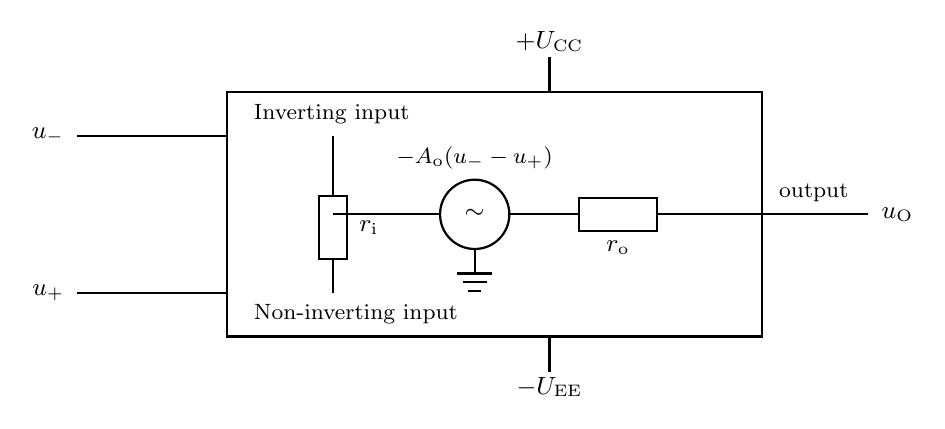
\begin{tikzpicture}[line width=0.8pt,scale=1.0,font=\small,
    every node/.append style={inner sep=1.5pt}]
  \draw (0,0) rectangle (6.80,3.10);
  % 输入电阻
  \draw (1.35,2.55)--(1.35,1.78);
  \draw[fill=white] (1.17,1.78) rectangle (1.53,0.98);
  \draw (1.35,0.98)--(1.35,0.55);
  \node[anchor=west] at (1.62,1.38) {$r_{\mathrm{i}}$};
  % 输入端子
  \draw (-1.90,2.55)--(0,2.55);
  \node[anchor=east] at (-2.00,2.55) {$u_-$};
  \node[anchor=west] at (0.28,2.82) {\footnotesize Inverting input};
  \draw (-1.90,0.55)--(0,0.55);
  \node[anchor=east] at (-2.00,0.55) {$u_+$};
  \node[anchor=west] at (0.28,0.28) {\footnotesize Non-inverting input};
  % 受控源
  \draw (3.15,1.55) circle (0.44);
  \node at (3.15,1.55) {$\sim$};
  \node[anchor=south] at (3.15,2.06) {\footnotesize $-A_{\mathrm{o}}(u_--u_+)$};
  \draw (4.47,1.55)--(3.59,1.55);
  \draw (1.35,1.55)--(2.71,1.55);
  \draw (3.15,1.11)--(3.15,0.80);
  \draw (2.93,0.80)--(3.37,0.80);
  \draw (3.00,0.69)--(3.30,0.69);
  \draw (3.07,0.58)--(3.23,0.58);
  % 输出电阻
  \draw[fill=white] (4.47,1.76) rectangle (5.47,1.34);
  \draw (5.47,1.55)--(6.80,1.55);
  \node[anchor=north] at (4.97,1.28) {$r_{\mathrm{o}}$};
  % 输出端子
  \draw (6.80,1.55)--(8.15,1.55);
  \node[anchor=west] at (8.25,1.55) {$u_{\mathrm{O}}$};
  \node[anchor=west] at (6.95,1.82) {\footnotesize output};
  % 电源
  \draw (4.10,3.10)--(4.10,3.55);
  \node[anchor=south] at (4.10,3.55) {$+U_{\mathrm{CC}}$};
  \draw (4.10,0)--(4.10,-0.45);
  \node[anchor=north] at (4.10,-0.45) {$-U_{\mathrm{EE}}$};
\end{tikzpicture}

\small 图 1-2\quad 运放等效电路（按 p13 重绘）：输入端是一只 $r_{\mathrm{i}}$，输出端是
\textbf{一个受控电压源与 $r_{\mathrm{o}}$ 串联}；受控源的电压是 $-A_{\mathrm{o}}(u_--u_+)$。
\end{center}

读这张图要读出三件事：

\begin{enumerate}
\item \textbf{输出与输入的连接被切断}：除受控源之外，输出端与输入端之间没有任何通路。
所以「输入决定输出」全靠那个受控源，\textbf{单向}——这正是 §5 里能把「信号从输入到输出、再从输出回到输入」
分成两条独立路径的前提。
\item \textbf{受控源的电压是差的函数}：$-A_{\mathrm{o}}(u_--u_+)$ 与 $A_{\mathrm{o}}(u_+-u_-)$ 是同一个数
（差一个负号两次），所以全章统一写成
\[
u_{\mathrm{O}}=A_{\mathrm{o}}\,(u_+-u_-)=A_{\mathrm{o}}u_{\mathrm{D}} .
\]
\item \textbf{两个电阻的位置决定两件事}：$r_{\mathrm{i}}$ 在输入端，决定「会不会从信号源吃电流」
（§7 的虚断就来自它）；$r_{\mathrm{o}}$ 与受控源串联在输出端，决定「带负载后输出会不会掉」
（p50 的 $u_{\mathrm{OL}}=u_{\mathrm{OC}}$ 就来自它）。
\end{enumerate}

\subhdr{p14 那道题：3000 V 去哪了}

p14 在等效电路旁边放了一道题，原文只有一句：
\textit{If $u_{\mathrm{D}}=3\ \mathrm{mV}$, $A_{\mathrm{o}}=10^{6}$. Find the output of Op Amp.}
下标还给了式子 $u_{\mathrm{O}}=-A_{\mathrm{O}}(u_- - u_+)=A_{\mathrm{O}}u_{\mathrm{D}}$。
\textbf{课件只问不答}，这里把它算完，因为它正好是 §2 的引子。

代入：
\[
u_{\mathrm{O}}=A_{\mathrm{o}}u_{\mathrm{D}}=10^{6}\times 3\times10^{-3}\ \mathrm{V}=3000\ \mathrm{V}.
\]

三千伏显然出不来。原因不是公式错，而是\textbf{公式只在没饱和时成立}：电源只有 $\pm U_{\mathrm{CC}}$
（典型 $\pm15\ \mathrm{V}$，p22 的例子用 $\pm12\ \mathrm{V}$、$\pm6\ \mathrm{V}$），
输出最高只能到 $+U_{\mathrm{OM}}$、最低只能到 $-U_{\mathrm{OM}}$。所以这道题的\textbf{正确答案是 $+U_{\mathrm{OM}}$
（p22 的例子会直接写成 $+12\ \mathrm{V}$），而不是 $3000\ \mathrm{V}$}。

\begin{wbx}
这一步是本章最容易丢分的地方：\textbf{$u_{\mathrm{O}}=A_{\mathrm{o}}u_{\mathrm{D}}$ 是「线性区」里的关系，
不是万能公式。}算出来的值一旦超过 $\pm U_{\mathrm{OM}}$，就必须改口说「饱和在 $\pm U_{\mathrm{OM}}$」。
3 mV 的净输入就把输出顶出 3000 V，说明运放的线性区\textbf{极其窄}——窄到什么程度，§2.3 会算出具体数字。
\end{wbx}

%=============================================================
\hdr{§2}{5.2 电压传输特性：一条被「夹」住的直线}

\subhdr{定义：输出是净输入的函数（p15）}

p15 给的定义是
\[
u_{\mathrm{O}}=f(u_{\mathrm{D}})=f(u_+-u_-),
\]
即把 $u_{\mathrm{D}}$ 当横轴、$u_{\mathrm{O}}$ 当纵轴画出来的那条曲线（\textbf{电压传输特性}）。
注意这条曲线\textbf{与输入信号的频率无关}，它描述的是「直流或极慢变化下，输出跟着净输入怎么变」，
所以叫「传输特性」而不是「频率特性」。

\subhdr{三段：线性区、正向饱和、负向饱和（p16--p19）}

p16--p19 用四页把这条曲线一段一段点亮，p20 再把「$A_{\mathrm{o}}$ 越大越陡」画出来。
下面这张图把四页合成一张，并标出三个区与两个分界点：

\begin{center}
\begin{tikzpicture}[line width=0.9pt,scale=1.0,font=\small,every node/.append style={inner sep=1.5pt}]
  % 坐标轴
  \draw[-{Latex}] (-4.6,0)--(4.6,0) node[anchor=west] {$u_{\mathrm{D}}$};
  \draw[-{Latex}] (0,-3.1)--(0,3.3) node[anchor=south] {$u_{\mathrm{O}}$};
  \node[anchor=north east] at (-0.12,-0.05) {$0$};
  % 三段
  \draw[very thick,violet] (-4.4,-2.2)--(-0.62,-2.2);
  \draw[very thick,violet] (4.4,2.2)--(0.62,2.2);
  \draw[very thick,violet] (-0.62,-2.2)--(0.62,2.2);
  % 分界虚线
  \draw[dashed,inkgray] (0.62,2.2)--(0.62,0);
  \draw[dashed,inkgray] (-0.62,-2.2)--(-0.62,0);
  % 标注
  \draw[dashed,inkgray] (-4.4,2.2)--(0,2.2);
  \draw[dashed,inkgray] (-4.4,-2.2)--(0,-2.2);
  \node[anchor=east] at (-0.10,2.20) {$+U_{\mathrm{OM}}$};
  \node[anchor=east] at (-0.10,-2.20) {$-U_{\mathrm{OM}}$};
  \node[anchor=north] at (0.62,-0.12) {\footnotesize $+\dfrac{U_{\mathrm{OM}}}{A_{\mathrm{o}}}$};
  \node[anchor=north] at (-0.70,-0.12) {\footnotesize $-\dfrac{U_{\mathrm{OM}}}{A_{\mathrm{o}}}$};
  \node[anchor=west] at (0.85,1.55) {\footnotesize 线性区（斜率 $A_{\mathrm{o}}$）};
  \node[anchor=west] at (-4.3,1.35) {\footnotesize 正向饱和区};
  \node[anchor=west] at (-4.3,-1.90) {\footnotesize 负向饱和区};
  \node[anchor=west] at (-4.3,2.55) {\footnotesize $u_{\mathrm{O}}=+U_{\mathrm{OM}}\approx+U_{\mathrm{CC}}$};
  \node[anchor=west] at (-4.3,-2.85) {\footnotesize $u_{\mathrm{O}}=-U_{\mathrm{OM}}\approx-U_{\mathrm{EE}}$};
\end{tikzpicture}

\small 图 2-1\quad 电压传输特性（按 p16--p20 重绘）。三段：$u_{\mathrm{D}}>\frac{U_{\mathrm{OM}}}{A_{\mathrm{o}}}$ 时
输出被夹在 $+U_{\mathrm{OM}}$；$u_{\mathrm{D}}<-\frac{U_{\mathrm{OM}}}{A_{\mathrm{o}}}$ 时夹在 $-U_{\mathrm{OM}}$；
中间那一段才是 $u_{\mathrm{O}}=A_{\mathrm{o}}u_{\mathrm{D}}$。
\end{center}

三段对应课件三句话：p17 的 \textit{Linear zone: $u_{\mathrm{O}}=A_{\mathrm{o}}u_{\mathrm{D}}$}、
p18 的 \textit{Positive saturation zone: $u_{\mathrm{O}}=+U_{\mathrm{OM}}\approx+U_{\mathrm{CC}}$}、
p19 的 \textit{Negative saturation zone: $u_{\mathrm{O}}=-U_{\mathrm{OM}}\approx-U_{\mathrm{EE}}$}。

p19 还并列了五个设问（\textit{Where is the linear zone? / What is the positive saturation voltage?}…），
本讲义把答案直接写在图上：线性区在 $\left|u_{\mathrm{D}}\right|<U_{\mathrm{OM}}/A_{\mathrm{o}}$，
正向、负向饱和电压分别是 $+U_{\mathrm{OM}}$、$-U_{\mathrm{OM}}$。

\subhdr{线性区窗口到底多窄：把数代进去}

这是本节最该动手算的一步，课件没有算。取 p10 的实际参数 $A_{\mathrm{o}}=10^{6}$、
p22 的电源 $\pm12\ \mathrm{V}$（即 $U_{\mathrm{OM}}\approx12\ \mathrm{V}$），线性区的半宽是
\[
\left|u_{\mathrm{D}}\right|<\frac{U_{\mathrm{OM}}}{A_{\mathrm{o}}}
=\frac{12}{10^{6}}\ \mathrm{V}=12\ \mu\mathrm{V}.
\]

十二微伏。这就是 p14 那道题「3 mV 就顶出 3000 V」的定量版本：
\textbf{净输入超过 12 $\mu\mathrm{V}$，输出就饱和}。这个数字解释了两件事：

\begin{itemize}
\item \textbf{开环不能当放大器}。想让输出在 $\pm12\ \mathrm{V}$ 之间连续变化，就得把净输入控制在
$\pm12\ \mu\mathrm{V}$ 以内——手动调不出来，环境温度漂一点就出界了。所以 p21 说开环运放只能当
\textbf{比较器}（§3）：它只回答「$u_+$ 比 $u_-$ 大还是小」，不回答「大多少」。
\item \textbf{必须用负反馈}。反馈的作用不是「让增益变大」（恰恰相反，它让增益变小），
而是\textbf{把输入端的差自动压到接近零}，让运放一直待在这条窄缝里。压得越狠，工作点越稳。
\end{itemize}

\aside{这里说的「12 $\mu\mathrm{V}$ 的缝」用的是\textbf{实际}运放的 $A_{\mathrm{o}}=10^{6}$。课件 p20 画的理想情形是
$A_{\mathrm{o}}\to\infty$，此时缝宽 $\to0$，直线变成\textbf{垂直}的一竖，
于是特性只剩两个值 $\pm U_{\mathrm{OM}}$——那就是一个理想比较器（§3）。}

\subhdr{p20：$A_{\mathrm{o}}$ 越大，那条线越陡}

p20 左右两图，左边是实际运放（斜率有限），右边是理想运放（竖直），配两句话：
\textit{The bigger the $A_{\mathrm{o}}$, the steeper the straight line will be.}
与 \textit{For ideal Op Amp the line is vertical, because $A_{\mathrm{o}}\to\infty$.}

这两句话是本节的落点：\textbf{把 $A_{\mathrm{o}}$ 当无穷大，传输特性就退化成一段竖线 + 两段水平线}。
竖线意味着「$u_+=u_-$ 时输出可以取任何值」，两段水平线意味着「只要 $u_+\neq u_-$，输出就顶到电源」。
§7 的\textbf{虚短}就是这条竖线的另一种说法：在线性区里，$u_+$ 与 $u_-$ 必须相等，
否则输出早就跑到饱和区去了。

%=============================================================
\hdr{§3}{5.3 比较器：开环运放的「二值」行为}

\subhdr{原理（p21）：两句话推出来}

p21 的原文给结论：
\textit{In an open-loop configuration, an ideal operational amplifier (op amp) behave as a comparator.
The behavior of op amp as a comparator is due to infinite open-loop gain. When it is working as a
comparator, there are only two outputs possible at the output of op amp.}
后面两句是半个推导：
\textit{If $u_+>u_-$ the output will be positive; if $u_+<u_-$ the output will be negative.}

这里把「为什么只有两个值」补完整，用的全是 §2 的图，不引入新东西：

\begin{enumerate}
\item 开环时输出与输入之间没有反馈通路，$u_+$ 与 $u_-$ 由外部两个电压\textbf{各自决定}，
两者之差 $u_{\mathrm{D}}$ 一般\textbf{不会}恰好落在那条 $12\ \mu\mathrm{V}$ 的缝里。
\item 只要 $u_{\mathrm{D}}$ 出了缝，§2 的传输特性就把它判到两段水平线之一：
$u_{\mathrm{D}}>0$ 落正向饱和（$+U_{\mathrm{OM}}$），$u_{\mathrm{D}}<0$ 落负向饱和（$-U_{\mathrm{OM}}$）。
\item 理想运放的缝宽为零，所以\textbf{除了 $u_+=u_-$ 这一个点，输出只有 $+U_{\mathrm{OM}}$ 与 $-U_{\mathrm{OM}}$ 两种可能}。
\end{enumerate}

于是判据极其简单，一句话：
\[
u_+>u_-\ \Longrightarrow\ u_{\mathrm{O}}=+U_{\mathrm{OM}},\qquad
u_+<u_-\ \Longrightarrow\ u_{\mathrm{O}}=-U_{\mathrm{OM}} .
\]
注意判据里\emph{没有} $A_{\mathrm{o}}$、没有电阻、没有线性区——比较器电路里\textbf{没有反馈}，
所以 §7 的虚短虚断在这里\textbf{一条也不成立}。这一点很多人在做 §5 的判定题时会搞混。

\subhdr{四道例题（p22）逐题判}

p22 并排放四个比较器电路，每个都用理想运放符号（$\infty$）、单电源标注为 $\pm12\ \mathrm{V}$ 或 $\pm6\ \mathrm{V}$，
两个输入端各给一个直流电压。课件在 \ding{172}\ding{173} 上直接给出了答案（$+12\ \mathrm{V}$、$-6\ \mathrm{V}$），
\ding{174}\ding{175} 只画了电路、没给答案。四道题一起看图 3-1：

\begin{center}
\begin{tabular}{@{}c@{\hspace{0.55cm}}c@{}}
\cmpfig{$3\,\mathrm{V}$}{$4\,\mathrm{V}$}{$\pm12\,\mathrm{V}$}{$+12\,\mathrm{V}$}{0}
&
\cmpfig{$0.5\,\mathrm{V}$}{$0.3\,\mathrm{V}$}{$\pm6\,\mathrm{V}$}{$-6\,\mathrm{V}$}{0}
\\[10pt]
\cmpfig{$0.3\,\mathrm{V}$}{$0.5\,\mathrm{V}$}{$\pm6\,\mathrm{V}$}{$+6\,\mathrm{V}$}{1}
&
\cmpfig{$-0.3\,\mathrm{V}$}{$-0.5\,\mathrm{V}$}{$\pm6\,\mathrm{V}$}{$-6\,\mathrm{V}$}{2}
\\
\end{tabular}

\small 图 3-1\quad 比较器四例（按 p22 重绘）。图中四个电路依次是 \ding{172}\ding{173}\ding{174}\ding{175}；
每只运放都开环、按理想（$\infty$）画，上方圆圈是电源引脚并标出电源电压，
右侧方框是本讲义算出的输出值（\ding{172}\ding{173} 与课件给的答案一致，\ding{174}\ding{175} 课件未给）。
\ding{174}\ding{175} 的输出端还挂了两只\textbf{反并}的二极管，一只普通管、一只发光二极管（LED）；
二极管符号实心的是 LED，箭头方向表示「正向电流」的方向，不表示发光方向。
\end{center}

逐题的判读只用到一条判据 $u_+\gtrless u_-\Rightarrow$ 输出取哪个饱和值：

\begin{center}
\small
\begin{tabular}{@{}p{0.9cm}p{2.5cm}p{2.4cm}p{2.6cm}p{1.6cm}p{3.6cm}@{}}
\toprule
\thead{题} & \thead{$u_-$} & \thead{$u_+$} & \thead{$u_{\mathrm{D}}=u_+-u_-$} & \thead{$u_{\mathrm{O}}$} & \thead{附加现象}
\\
\midrule
\ding{172} & $3\ \mathrm{V}$ & $4\ \mathrm{V}$ & $+1\ \mathrm{V}>0$ & $+12\ \mathrm{V}$ & 电源 $\pm12\ \mathrm{V}$，无负载
\\
\ding{173} & $0.5\ \mathrm{V}$ & $0.3\ \mathrm{V}$ & $-0.2\ \mathrm{V}<0$ & $-6\ \mathrm{V}$ & 电源 $\pm6\ \mathrm{V}$
\\
\ding{174} & $0.3\ \mathrm{V}$ & $0.5\ \mathrm{V}$ & $+0.2\ \mathrm{V}>0$ & $+6\ \mathrm{V}$ & LED 正向导通、发光
\\
\ding{175} & $-0.3\ \mathrm{V}$ & $-0.5\ \mathrm{V}$ & $-0.2\ \mathrm{V}<0$ & $-6\ \mathrm{V}$ & LED 正向导通、发光
\\
\bottomrule
\end{tabular}
\end{center}

上面这张表只是把图 3-1 的四个电路按「$u_+$ 减 $u_-$ 的正负」读了一遍，逐行读法如下：

\begin{itemize}
\item \textbf{\ding{172}}：$u_+ = 4\ \mathrm{V}$ 高于 $u_- = 3\ \mathrm{V}$，净输入为正，输出取正向饱和。
电源是 $\pm12\ \mathrm{V}$，所以 $+U_{\mathrm{OM}}=+12\ \mathrm{V}$——与课件给的答案一致。
\item \textbf{\ding{173}}：$u_+ = 0.3\ \mathrm{V}$ 低于 $u_- = 0.5\ \mathrm{V}$，净输入为负，输出取负向饱和
$-U_{\mathrm{OM}} = -6\ \mathrm{V}$——与课件给的答案一致。
\item \textbf{\ding{174}}：这一题的 $\pm6\ \mathrm{V}$ 接法与 \ding{173} 相同，但两个输入电压\textbf{对调}了：
现在 $u_+ = 0.5\ \mathrm{V}$ 高于 $u_- = 0.3\ \mathrm{V}$，所以输出\textbf{翻到另一边}，取 $+6\ \mathrm{V}$。
输出端的 LED 接法是「阳极朝输出、阴极朝地」，$u_{\mathrm{O}}=+6\ \mathrm{V}$ 正好让它正向导通、发光；
另一只普通二极管反接（阳极朝地），此时截止。
\item \textbf{\ding{175}}：两个输入都取负值，$u_+=-0.5\ \mathrm{V}$ 低于 $u_-=-0.3\ \mathrm{V}$，输出取 $-6\ \mathrm{V}$。
\ding{175} 的 LED 与 \ding{174} 的接法相反（阳极朝地、阴极朝输出），所以这次是它正向导通、发光，普通管截止。
\end{itemize}

\warnbox{\textbf{\ding{174}\ding{175} 与 \ding{172}\ding{173} 的区别不只是「换个数」}：\ding{172}\ding{173} 只看输出电压，输出端什么都没接；
\ding{174}\ding{175} 在输出端挂了\textbf{两只反并的二极管}，于是「输出是高还是低」多了一层可见后果——
哪只管子导通，要看它的\textbf{阳极是否朝高电位}。这类题干问的往往不是电压值，而是
「哪只灯亮」。判读顺序固定：先定 $u_{\mathrm{O}}$ 的高低，再逐只看管子的阳极朝哪边。
（本讲义把图重绘时保留了原图的二极管朝向，箭头只标「正向电流」方向，不标发光方向。）}

\subhdr{两个边界，考试会踩}

\begin{enumerate}
\item \textbf{饱和电压与电源电压：课件用「$\approx$」，例题用「$=$」。}
p18、p19 写的是 $u_{\mathrm{O}}=+U_{\mathrm{OM}}\approx+U_{\mathrm{CC}}$、$u_{\mathrm{O}}=-U_{\mathrm{OM}}\approx-U_{\mathrm{EE}}$，
用的是约等号；p22 的四道例题却直接取 $+12\ \mathrm{V}$、$-6\ \mathrm{V}$。差别在哪：
真实运放的输出级是三极管，导通时总有一点压降，$U_{\mathrm{OM}}$ 通常比电源低 $1\sim2\ \mathrm{V}$；
课件的例题按\textbf{理想}算（当成等于电源），因为用 $\pm12\ \mathrm{V}$ 电源标出「$+12\ \mathrm{V}$」好判卷。
\textbf{做题时按题目的口径}：题里给了电源电压又没说 $U_{\mathrm{OM}}$ 的具体值，就取等于电源；
若题里另外给了 $U_{\mathrm{OM}}$，以 $U_{\mathrm{OM}}$ 为准。
\item \textbf{$u_+=u_-$ 那一点怎么算。}理想运放的传输特性是一条竖线，$u_{\mathrm{D}}=0$ 时输出
\textbf{不可确定}（理论上可以取 $\pm U_{\mathrm{OM}}$ 之间任何值，实际由器件失调决定）。
所以出题不会让两个输入端恰好相等；一旦遇到，要补一句「此时输出不确定」，
不能硬算出一个值。
\end{enumerate}




%=============================================================
\hdr{§4}{5.5.1 反馈的基本概念：把输出送回输入端}

\subhdr{定义（p23）}

p23 给的定义原文是：
\textit{Feedback: part or all of the output of the amplification circuit is brought back to the
input loop in a certain way to affect the input.}
（反馈：把放大电路输出的\textbf{一部分或全部}，按\textbf{一定的方式}送回\textbf{输入回路}，去\textbf{影响输入}。）

这一句里有四个要点，逐个落到本题：

\begin{itemize}
\item \textbf{「一部分或全部」}：全部送回去就是 100\% 反馈（输出直接连回输入端，电压跟随器就是这种）；
送一部分就是经一个\textbf{反馈网络}（通常由两三只电阻组成的分压器）取回一个比例。
\item \textbf{「一定的方式」}：送回的位置可以是反相端，也可以在同相端；可以与输入串联，也可以并联。
这句含糊的「一定的方式」，正是 §5.2--§5.4 要判的三件事。
\item \textbf{「送回输入回路」}：必须\textbf{回到输入端}、参与「输入与反馈的比较」才算反馈。
只在输出端挂一只电压表看着，不叫反馈。
\item \textbf{「影响输入」}：反馈的定义里就写明了它的效果——改变净输入的大小，这是 §5.2 判正负的依据。
\end{itemize}

p23 底部三张小图正好是这三句话的图示（本讲义按原图画法重绘，标出各自的接法）：

\begin{center}
\begin{tikzpicture}[line width=0.8pt,scale=0.85,font=\small,
    every node/.append style={inner sep=1.4pt}]
  % ---- \ding{172} 无反馈
  \begin{scope}[shift={(0,0)}]
    \draw (0,0) rectangle (1.8,1.9);
    \node[anchor=west] at (0.10,1.40) {$-$};
    \node[anchor=west] at (0.10,0.50) {$+$};
    \node at (1.10,0.95) {\footnotesize $A_{\mathrm{o}}$};
    \fill (1.30,1.53)--(1.44,1.60)--(1.30,1.67)--cycle;
    \draw (-2.0,1.40)--(0,1.40);
    \node[anchor=east] at (-2.1,1.40) {$u_{\mathrm{I}}$};
    \draw (-1.05,0.50)--(0,0.50);
    \draw (-1.05,0.50)--(-1.05,0.30);
    \draw (-1.20,0.30)--(-0.90,0.30);
    \draw (-1.15,0.19)--(-0.95,0.19);
    \draw (1.80,0.95)--(2.9,0.95);
    \node[anchor=west] at (2.45,1.20) {$u_{\mathrm{O}}$};
    \node[anchor=north] at (0.90,-0.30) {\ding{172}\ 无反馈（开环）};
  \end{scope}
  % ---- \ding{173} 输出全部回到反相端
  \begin{scope}[shift={(5.0,0)}]
    \draw (0,0) rectangle (1.8,1.9);
    \node[anchor=west] at (0.10,1.40) {$-$};
    \node[anchor=west] at (0.10,0.50) {$+$};
    \node at (1.10,0.95) {\footnotesize $A_{\mathrm{o}}$};
    \fill (1.30,1.53)--(1.44,1.60)--(1.30,1.67)--cycle;
    \draw (-2.0,1.40)--(0,1.40);
    \node[anchor=east] at (-2.1,1.40) {$u_{\mathrm{I}}$};
    \draw (-1.05,0.50)--(0,0.50);
    \draw (-1.05,0.50)--(-1.05,0.30);
    \draw (-1.20,0.30)--(-0.90,0.30);
    \draw (-1.15,0.19)--(-0.95,0.19);
    \draw (1.80,0.95)--(2.9,0.95);
    \node[anchor=west] at (2.45,1.20) {$u_{\mathrm{O}}$};
    % 反馈：从输出直接回到反相端
    \draw (2.35,0.95)--(2.35,2.55)--(-1.25,2.55)--(-1.25,1.40);
    \node[anchor=north] at (0.90,-0.30) {\ding{173}\ 输出全部回到反相端};
  \end{scope}
  % ---- \ding{174} 经反馈网络回到同相端
  \begin{scope}[shift={(10.0,0)}]
    \draw (0,0) rectangle (1.8,1.9);
    \node[anchor=west] at (0.10,1.40) {$-$};
    \node[anchor=west] at (0.10,0.50) {$+$};
    \node at (1.10,0.95) {\footnotesize $A_{\mathrm{o}}$};
    \fill (1.30,1.53)--(1.44,1.60)--(1.30,1.67)--cycle;
    \draw (-2.0,1.40)--(0,1.40);
    \node[anchor=east] at (-2.1,1.40) {$u_{\mathrm{I}}$};
    \draw (1.80,0.95)--(2.9,0.95);
    \node[anchor=west] at (2.45,1.20) {$u_{\mathrm{O}}$};
    % 反馈：从输出经反馈网络回到同相端
    \draw (2.35,0.95)--(2.35,-0.55)--(0.55,-0.55);
    \draw[fill=white] (0.05,-0.72) rectangle (0.55,-0.38);
    \draw (0.05,-0.55)--(-1.05,-0.55)--(-1.05,0.50)--(0,0.50);
    \draw (-1.05,-0.55)--(-1.05,-0.85);
    \draw (-1.20,-0.85)--(-0.90,-0.85);
    \draw (-1.15,-0.96)--(-0.95,-0.96);
    \node[anchor=north] at (0.90,-1.20) {\ding{174}\ 经反馈网络回到同相端};
  \end{scope}
\end{tikzpicture}

\small 图 4-1\quad 反馈的三种接法（按 p23 重绘）：\ding{172} 没有反馈，输出与输入之间没有通路；
\ding{173} 输出经一根导线\textbf{全部}送回到\textbf{反相端}（这就是电压跟随器）；
\ding{174} 输出经一个\textbf{反馈网络}（灰色方框，这里是分压电阻）把\textbf{一部分}送回，落在\textbf{同相端}。
\end{center}

\aside{按 §5.2 的判据可以马上验证：\ding{173} 反馈回到反相端 $\Rightarrow$ 负反馈；
\ding{174} 反馈回到同相端 $\Rightarrow$ 正反馈。课件把这两张图放在「定义」页，是为了说明「接法可以不同」，
而不是说它们都合理——正反馈那一种在放大电路里是要避免的（§6.1 会说明为什么）。}

\subhdr{开环与闭环（p24）}

p24 用两句话把两个术语定死：
\textit{Open-loop: When a system does not have the feedback structure, it is called an open-loop
system, which is the simplest and most economical type of control system.}
\textit{Closed-loop: A system with one or more feedback paths.}

中文：\textbf{开环}＝没有反馈通路，结构最简单、最经济；\textbf{闭环}＝有一条或多条反馈通路。
注意「开环 / 闭环」说的是\textbf{有没有反馈通路}，不是「增益大不大」：
§3 的比较器是开环，§5 的判定题里八道题全是闭环。

\subhdr{框图与三个系数（p25--p26）}

p26 把反馈系统抽象成一个框图：输入 $x_{\mathrm{I}}$ 进比较环节，与反馈信号 $x_{\mathrm{F}}$ 相减得到
净输入 $x_{\mathrm{D}}$，再经放大器 $A_{\mathrm{o}}$ 得到输出 $x_{\mathrm{O}}$；输出经反馈网络 $F$ 变成 $x_{\mathrm{F}}$ 回到比较环节。

\begin{center}
\begin{tikzpicture}[line width=0.8pt,scale=1.0,font=\small,
    every node/.append style={inner sep=1.5pt},>=Latex]
  % 主通路
  \draw[->] (-4.6,0)--(-1.55,0);
  \node[anchor=north] at (-2.9,0.02) {$x_{\mathrm{I}}$};
  \node[anchor=south] at (-4.2,0.10) {\footnotesize 输入};
  \draw (0,0) circle (0.42);
  \draw (-0.22,-0.22)--(0.22,0.22);
  \draw (-0.22,0.22)--(0.22,-0.22);
  \draw[->] (0.44,0)--(2.0,0);
  \node[anchor=north] at (1.2,0.02) {$x_{\mathrm{D}}$};
  \node[anchor=south] at (1.2,0.10) {\footnotesize 净输入};
  \draw (2.0,-0.62) rectangle (4.3,0.62);
  \node at (3.15,0.14) {\footnotesize 放大};
  \node at (3.15,-0.22) {$A_{\mathrm{o}}$};
  \draw[->] (4.3,0)--(6.4,0);
  \node[anchor=north] at (5.3,0.02) {$x_{\mathrm{O}}$};
  \node[anchor=south] at (5.3,0.10) {\footnotesize 输出};
  % 反馈通路
  \draw (5.7,0)--(5.7,-2.3)--(4.3,-2.3);
  \draw[->] (4.3,-2.3)--(3.7,-2.3);
  \draw (1.2,-2.92) rectangle (3.7,-1.68);
  \node at (2.45,-2.14) {\footnotesize 反馈};
  \node at (2.45,-2.52) {$F$};
  \draw[->] (1.2,-2.3)--(-0.42,-2.3);
  \node[anchor=east] at (0.4,-2.54) {$x_{\mathrm{F}}$};
  \node[anchor=west] at (0.55,-2.06) {\footnotesize 反馈信号};
  \draw[->] (-0.42,-2.3)--(-0.42,-0.42);
\end{tikzpicture}

\small 图 4-2\quad 反馈系统的框图（按 p25、p26、p44 重绘）。比较环节画成带叉的圆圈（课件用的就是这个符号），
它把 $x_{\mathrm{I}}$ 与 $x_{\mathrm{F}}$ \textbf{相减}；反馈网络 $F$ 从输出取样、送回到比较环节。
\end{center}

p26 在框图旁边给出三个系数，本讲义按原式抄下：
\[
A_{\mathrm{o}}=\frac{x_{\mathrm{O}}}{x_{\mathrm{D}}}\ \ \text{（开环增益）},\qquad
A_{\mathrm{F}}=\frac{x_{\mathrm{O}}}{x_{\mathrm{I}}}\ \ \text{（闭环增益）},\qquad
F=\frac{x_{\mathrm{F}}}{x_{\mathrm{O}}}\ \ \text{（反馈系数）}.
\]

\begin{wbx}
\textbf{注意 $x$ 不是电压的专属符号。}框图里 $x$ 可以是电压也可以是电流，取决于「取什么量来比较」：
比较的是电压，$x$ 就是 $u$；比较的是电流，$x$ 就是 $i$。这就是 §5.4「串联/并联」那一维的意义：
串联时比较电压，并联时比较电流。所以 $A_{\mathrm{o}}$ 在框图中叫「开环增益」而不叫「开环电压增益」，
只有当 $x$ 确实取了电压，它才是电压增益——课件 p26 的标题写 \textit{Open loop voltage gain}，
那是把它当成电压增益来称呼的习惯写法。
\end{wbx}

框图里还有一个式子没有单独编号，但它是后面所有推导的起点：
\[
x_{\mathrm{D}}=x_{\mathrm{I}}-x_{\mathrm{F}} .
\]
\textbf{减号}是「比较环节」这个圆圈带来的，也\textbf{正是负反馈的约定}：反馈信号被从输入里扣掉。
§6.1 推闭环增益时从它出发；§5.2 判正负时，判的其实就是「这个减号在具体电路里到底是不是在减」。

%=============================================================
\hdr{§5}{5.5.2 反馈的类型：三个维度、三条判据、八道题}

\subhdr{三个维度（p27）}

p27 把反馈分成三类，每一类都是一个「是哪一个」的问题：

\begin{enumerate}
\item \textbf{Positive or negative}（正还是负）：\textit{Whether the feedback has the same effect as the input.}
反馈的效果与输入\textbf{相同}（让净输入变大）还是\textbf{相反}（让净输入变小）？
\item \textbf{Voltage or current}（电压还是电流）：\textit{Whether the feedback is taken from the output
voltage or current.} 反馈信号取自\textbf{输出电压}还是\textbf{输出电流}？
\item \textbf{Series or parallel}（串联还是并联）：\textit{Whether the feedback is connected in series
or parallel with the input.} 反馈在输入端与输入信号\textbf{串联}（比较电压）还是\textbf{并联}（比较电流）？
\end{enumerate}

三个维度各问一件事，\textbf{互相独立}，所以一个反馈电路可以用三个词描述完，例如
「电压并联负反馈」「电流串联正反馈」。三个维度各两种取法，一共 $2\times2\times2=8$ 种组合——
这不是巧合：p36--p43 的八道判定题，正好把八种组合\textbf{各用一次}（§5.5 末会用一张表把这件事点明）。

\subhdr{判据一：正还是负（p28--p30）}

p28 给的判据是一句话：
\textit{PF: $x_{\mathrm{D}}$ is increased under the combined effect of $x_{\mathrm{I}}$ and $x_{\mathrm{F}}$；
NF: $x_{\mathrm{D}}$ is decreased under the combined effect of $x_{\mathrm{I}}$ and $x_{\mathrm{F}}$.}
（正反馈：在输入与反馈的共同作用下，\textbf{净输入增大}；负反馈：净输入\textbf{减小}。）

判据本身很简单，难在「怎么知道净输入是增大还是减小」。p29、p30 各给一个示范电路，用的都是同一个办法：
\textbf{瞬时极性法}——假设输入瞬时为正，沿放大器一路标极性，看反馈送回来的是同号还是反号。

p29 的示范电路（反馈回到\textbf{同相端}）与 p30 的示范电路（反馈回到\textbf{反相端}）如下：

\begin{center}
\begin{tabular}{@{}c@{\hspace{0.35cm}}c@{}}
\famcirc[pol]{2}{2}{1}{R_{2}}{R_{1}}{0.75}
&
\famcirc[pol]{2}{1}{2}{R_{2}}{R_{1}}{0.75}
\\[-6pt]
{\small (a) 课件 p29：反馈回到同相端} & {\small (b) 课件 p30：反馈回到反相端}
\end{tabular}

\small 图 5-1\quad 课件给的两个示范电路（按 p29、p30 重绘，只把「极性标记」画成三个 $\oplus$）。
两个电路的输入端都在\textbf{同相端}（$u_{\mathrm{I}}$ 经 $R_2$ 进「$+$」），区别只在 $R_{\mathrm{F}}$ 回到哪里：
(a) 与 $u_{\mathrm{I}}$ \textbf{落在同一个节点}上，(b) 落在\textbf{另一个端子}（反相端）上。
\end{center}

\textbf{(a) 的判读（p29）}：\ding{172}在 $u_{\mathrm{I}}$ 处标「$+$」；\ding{173}输入从同相端进，所以输出 $u_{\mathrm{O}}$ 也是「$+$」，
在输出端标「$+$」；\ding{174}$R_{\mathrm{F}}$ 把「$+$」送回\textbf{同相端}，而这个节点正是 $u_{\mathrm{I}}$ 进来的节点——
两路信号\textbf{同号相加}，净输入 $i_{\mathrm{D}}$ 被抬高。p29 的原文写
\textit{the feedback effective is to increase the net input $i_{\mathrm{D}}$}，即
\[
i_{\mathrm{D}}=i_{\mathrm{I}}+i_{\mathrm{F}} \quad\Longrightarrow\quad \text{正反馈}.
\]
注意 p29 用的是\textbf{电流}记号（$i_{\mathrm{I}}$、$i_{\mathrm{F}}$、$i_{\mathrm{D}}$）：因为输入与反馈落在同一个节点上，
比较的是「谁往这个节点里灌的电流多」，这正是 §5.4 的「并联」。

\textbf{(b) 的判读（p30）}：\ding{172}在 $u_{\mathrm{I}}$ 处标「$+$」；\ding{173}输入从同相端进，输出 $u_{\mathrm{O}}$ 为「$+$」；
\ding{174}$R_{\mathrm{F}}$ 把「$+$」送回\textbf{反相端}，于是反相端的电位被抬高。而
\[
u_{\mathrm{D}}=u_{\mathrm{I}}-u_{\mathrm{F}},
\]
$u_{\mathrm{F}}$ 抬高 $\Rightarrow$ $u_{\mathrm{D}}$ 减小 $\Rightarrow$ 净输入被抵削。p30 原文：
\textit{the net input $u_{\mathrm{D}}$ is reduced because $u_{\mathrm{F}}$ is increased. So the feedback is NF.}

\aside{(b) 里 $R_{\mathrm{F}}$ 的右端并不是接在输出端上，而是接在 $R_{\mathrm{L}}$ 与 $R$ 之间——这一点在判「电压/电流」时是关键（§5.3）。
读 (b) 的图时要看清：$R_{\mathrm{L}}$ 是负载，$R$ 是串在负载回路里的\textbf{取样电阻}，
所以 $u_{\mathrm{F}}$ 取自 $R$ 两端，它与输出电流成正比，而不是输出电压。}

两张图读完，可以把它压成一条\textbf{可复用的规则}——不用每次重走一遍极性传播：

\begin{cbox}
\textbf{极性规则}：反馈回到\textbf{反相端} $\Rightarrow$ \textbf{负反馈}；反馈回到\textbf{同相端} $\Rightarrow$ \textbf{正反馈}。
\end{cbox}

这条规则为什么对？把四种接法列全，逐行看「输入自己造成的影响」与「反馈造成的影响」是否同向。
表前一句：这张表只是把「$u_{\mathrm{I}}$ 与 $u_{\mathrm{F}}$ 各自对 $u_{\mathrm{D}}=u_+-u_-$ 的作用方向」在两处各读一次
（输入落在哪个端子决定 $u_{\mathrm{O}}$ 的极性，反馈落在哪个端子决定它抬高的是 $u_+$ 还是 $u_-$）。

\begin{center}
\small
\begin{tabular}{@{}p{2.4cm}p{2.4cm}p{3.4cm}p{4.2cm}p{1.7cm}@{}}
\toprule
\thead{输入落在} & \thead{反馈落在} & \thead{$u_{\mathrm{I}}\uparrow$ 时 $u_{\mathrm{O}}$} & \thead{反馈对净输入 $u_{\mathrm{D}}$ 的作用} & \thead{结论}
\\
\midrule
反相端 & 反相端 & 下降（$-$） & 把 $u_-$ 拉低 $\Rightarrow$ $u_{\mathrm{D}}$ 回升，抵削输入 & 负反馈
\\
反相端 & 同相端 & 下降（$-$） & 把 $u_+$ 拉低 $\Rightarrow$ $u_{\mathrm{D}}$ 更低，加强输入 & 正反馈
\\
同相端 & 反相端 & 上升（$+$） & 把 $u_-$ 抬高 $\Rightarrow$ $u_{\mathrm{D}}$ 更低，抵削输入 & 负反馈
\\
同相端 & 同相端 & 上升（$+$） & 把 $u_+$ 抬高 $\Rightarrow$ $u_{\mathrm{D}}$ 更高，加强输入 & 正反馈
\\
\bottomrule
\end{tabular}
\end{center}

逐行读法（每行只需看两处）：

\begin{itemize}
\item \textbf{第 1 行}：输入在反相端，所以 $u_{\mathrm{I}}$ 一抬高，$u_{\mathrm{D}}$ 就被压低、$u_{\mathrm{O}}$ 向下跑；
输出向下，经 $R_{\mathrm{F}}$ 回到\textbf{同一个}反相端节点，把那一点也往下拉——后者让 $u_{\mathrm{D}}$ 回升，
与输入的作用相反，抵削，故为负反馈。
\item \textbf{第 2 行}：输入在反相端（$u_{\mathrm{O}}$ 向下），反馈却落在同相端，把 $u_+$ 往下拉；
下端往下、上端不变，$u_{\mathrm{D}}$ 进一步降低，与输入同向，加强，故为正反馈。
\item \textbf{第 3 行}：输入在同相端（$u_{\mathrm{O}}$ 向上），反馈落在反相端，把 $u_-$ 往上抬，
$u_{\mathrm{D}}$ 被压低，与输入的作用相反，负反馈。
\item \textbf{第 4 行}：输入在同相端（$u_{\mathrm{O}}$ 向上），反馈也落在同相端，两路同号相加，正反馈。
\end{itemize}

边界行：四种接法里没有第五种（端子只有两个、输入与反馈各落其一），所以这条规则\textbf{覆盖全部情形}，
做 §5.5 的八道题时可以直接用。唯一要注意的是：这里的「抬高/拉低」说的是\textbf{瞬时变化的方向}，
不是绝对电位的高低——所以输入标的是「$+$」而不是某个具体电压值。

\subhdr{判据二：电压还是电流（p31--p32）}

p31 给判据，两条都写全：
\begin{itemize}
\item \textbf{令 $R_{\mathrm{L}}=0$（输出短路）}，则 $u_{\mathrm{O}}=0$。此时若反馈信号 $x_{\mathrm{F}}=0$，就是
\textbf{电压反馈（VF）}；否则是\textbf{电流反馈（CF）}。
\item \textbf{令 $R_{\mathrm{L}}=\infty$（输出开路）}，则 $i_{\mathrm{O}}=0$。此时若 $x_{\mathrm{F}}=0$，就是
\textbf{电流反馈（CF）}；否则是\textbf{电压反馈（VF）}。
\end{itemize}
p31 顶上还有一句定性的话：\textit{CF: $x_{\mathrm{F}}$ is proportional to $i_{\mathrm{O}}$;
VF: $x_{\mathrm{F}}$ is proportional to $u_{\mathrm{O}}$.}（电压反馈的反馈量与 $u_{\mathrm{O}}$ 成正比，
电流反馈的反馈量与 $i_{\mathrm{O}}$ 成正比。）

判据的\textbf{机制}一句话：\textbf{把负载短路，看反馈信号还在不在}。
反馈是按「输出端的某个量」成比例取回来的，所以短路后那个量没了，反馈就没了。

p32 用两个例子把两条判据各用一次，就是图 5-1 的那两个电路：

\begin{center}
\begin{tabular}{@{}c@{\hspace{0.35cm}}c@{}}
\famcirc{2}{2}{1}{R_{2}}{R_{1}}{0.75}
&
\famcirc{2}{1}{2}{R_{2}}{R_{1}}{0.75}
\\[-6pt]
{\small (a) 短路 $R_{\mathrm{L}}$ 后 $i_{\mathrm{F}}=0$ $\Rightarrow$ VF} & {\small (b) 短路 $R_{\mathrm{L}}$ 后 $u_{\mathrm{F}}\neq0$ $\Rightarrow$ CF}
\end{tabular}

\small 图 5-2\quad 电压/电流判别的两个示范（按 p32 重绘）。两图都是从左边做了一次「把 $R_{\mathrm{L}}$ 短路」的思想实验，
红笔把 $R_{\mathrm{L}}$ 划掉；区别在 $R_{\mathrm{F}}$ 的右端取在哪里。
\end{center}

\begin{itemize}
\item \textbf{(a)}：$R_{\mathrm{F}}$ 的右端直接接在\textbf{输出端}（$R_{\mathrm{L}}$ 的上端）。
把 $R_{\mathrm{L}}$ 短路 $\Rightarrow$ $u_{\mathrm{O}}=0$ $\Rightarrow$ $R_{\mathrm{F}}$ 两端的电压差塌掉、$i_{\mathrm{F}}=0$
$\Rightarrow$ 反馈消失 $\Rightarrow$ \textbf{电压反馈}。p32 原文：\textit{Output short-circuit: $R_{\mathrm{L}}=0$, $u_{\mathrm{O}}=0$.
The feedback $i_{\mathrm{F}}=0$, so it is VF.}
\item \textbf{(b)}：$R_{\mathrm{F}}$ 的右端接在 $R_{\mathrm{L}}$ 与 $R$ 之间的节点上，取的是 $R$ 两端的电压。
把 $R_{\mathrm{L}}$ 短路 $\Rightarrow$ $u_{\mathrm{O}}=0$，但 $R$ 上仍有电流流过（输出级还在往短路点灌电流），
$u_{\mathrm{F}}\neq0$ $\Rightarrow$ 反馈仍在 $\Rightarrow$ \textbf{电流反馈}。p32 原文：
\textit{Output short-circuit: $R_{\mathrm{L}}=0$, $u_{\mathrm{O}}=0$. The feedback $u_{\mathrm{F}}\neq0$, so it is CF.}
\end{itemize}

\aside{这里有一个反直觉之处值得点破：\textbf{「电流反馈」不等于「反馈量是电流」}。(b) 取回来的 $u_{\mathrm{F}}$ 明明是个电压，
为什么叫电流反馈？因为它与\textbf{输出电流}成正比（$u_{\mathrm{F}}=i_{\mathrm{O}}R$），
「电压/电流」说的是\textbf{取样对象}，不是反馈量本身的量纲。同理 (a) 的 $i_{\mathrm{F}}$ 虽然是个电流，
但它是输出电压 $u_{\mathrm{O}}$ 除以 $R_{\mathrm{F}}$ 得到的，与 $u_{\mathrm{O}}$ 成正比，所以叫电压反馈。}

把判据压成一条\textbf{看图就能用的规则}：

\begin{cbox}
\textbf{取样位置规则}：$R_{\mathrm{F}}$ 的右端接在\textbf{输出端}（和 $R_{\mathrm{L}}$ 上端同一个节点）$\Rightarrow$ \textbf{电压反馈}；
接在 $R_{\mathrm{L}}$ 与 $R$ 之间的节点（即 $R$ 的上端）$\Rightarrow$ \textbf{电流反馈}。
\textbf{先看有没有那只 $R$}：图里只有 $R_{\mathrm{L}}$ 一只下地电阻的，一定是电压反馈；
$R_{\mathrm{L}}$ 下面还串一只 $R$ 的，才可能是电流反馈。
\end{cbox}

\subhdr{判据三：串联还是并联（p33--p35）}

p33 给定义：\textbf{串联反馈（SF）}：反馈信号 $x_{\mathrm{F}}$ 与输入\textbf{串联}；
\textbf{并联反馈（PF）}：反馈信号 $x_{\mathrm{F}}$ 与输入\textbf{并联}。

p34 给判据（原文）：\textit{Point Q is short-circuited to the ground. If the input signal can still be
applied to the two input terminals of the amplifier, it is Series Feedback. Otherwise PF.}
（把 $Q$ 点接地。若输入信号仍能加到放大器的两个输入端，就是串联反馈；否则是并联反馈。）
$Q$ 点就是\textbf{反馈网络与输入回路的交点}。

这个判据的道理：串联时，输入与反馈是\textbf{两个独立的源}串在同一条路上（一个接在一个端子上、一个接在另一个端子上），
把反馈那个节点接地，输入还有自己的路可走；并联时，输入与反馈\textbf{并到同一个节点}上，
把这个节点接地，输入也被短路到地了，进不了放大器。

p35 的两个例子（图 5-1 的那两个电路，这次把 $Q$ 点标出来）：

\begin{center}
\begin{tabular}{@{}c@{\hspace{0.35cm}}c@{}}
\famcirc[q]{2}{2}{1}{R_{2}}{R_{1}}{0.75}
&
\famcirc[q]{2}{1}{2}{R_{2}}{R_{1}}{0.75}
\\[-6pt]
{\small (a) $Q$ 接地后 $u_{\mathrm{I}}$ 进不去 $\Rightarrow$ 并联} & {\small (b) $Q$ 接地后 $u_{\mathrm{I}}$ 仍能进来 $\Rightarrow$ 串联}
\end{tabular}

\small 图 5-3\quad 串联/并联判别的两个示范（按 p35 重绘）。$Q$ 标在「反馈网络与输入的交点」上：
(a) 的 $Q$ 就在同相端节点上，(b) 的 $Q$ 在反相端节点上，而输入走的是同相端。
\end{center}

\begin{itemize}
\item \textbf{(a)}：$Q$ 与「$u_{\mathrm{I}}$ 进放大器的那个节点」是\textbf{同一个点}。把它接地，$u_{\mathrm{I}}$ 经 $R_2$ 之后
被短路到地，进不了同相端 $\Rightarrow$ \textbf{并联}。p35 原文：
\textit{Point Q is grounded. $u_{\mathrm{I}}$ can not be applied to the input terminals, it is PF.}
\item \textbf{(b)}：$Q$ 在反相端，而 $u_{\mathrm{I}}$ 从同相端进——两条路\textbf{不共节点}。把 $Q$ 接地，
$u_{\mathrm{I}}$ 照样进得了同相端 $\Rightarrow$ \textbf{串联}。p35 原文：
\textit{Point Q is grounded. $u_{\mathrm{I}}$ can still be applied to the input terminals, it is SF.}
\end{itemize}

同一条规则再压一遍：

\begin{cbox}
\textbf{共节点规则}：反馈落点与输入落点\textbf{是同一个端子}（同一个节点）$\Rightarrow$ \textbf{并联}；
\textbf{不是同一个端子}（一个在反相端、一个在同相端）$\Rightarrow$ \textbf{串联}。
\end{cbox}

\aside{为什么「同一个节点」就是「并联」？因为同一节点上是\textbf{电流}在相加（基尔霍夫电流定律），
两路信号靠「谁的电流大」来比较；两个不同端子之间是\textbf{电压}在相减（$u_{\mathrm{D}}=u_+-u_-$），
靠「谁的电位高」来比较。这也解释了 §4 框图里 $x$ 为什么可以是电压也可以是电流：
串联对应电压比较，并联对应电流比较。}

\subhdr{三条判据为什么互不干扰}

三条判据各看一处\textbf{不同的事实}，所以可以分别判、答案可以任意组合：

\begin{center}
\small
\begin{tabular}{@{}p{2.6cm}p{4.6cm}p{8.0cm}@{}}
\toprule
\thead{维度} & \thead{看哪个位置} & \thead{判据}
\\
\midrule
正 / 负 & $R_{\mathrm{F}}$ 落在哪个\textbf{端子} & 反相端 $\Rightarrow$ 负反馈；同相端 $\Rightarrow$ 正反馈
\\
电压 / 电流 & $R_{\mathrm{F}}$ 的右端接在\textbf{哪个节点} & 输出端 $\Rightarrow$ 电压；$R_{\mathrm{L}}$ 与 $R$ 之间 $\Rightarrow$ 电流
\\
串联 / 并联 & 反馈端子与\textbf{输入端子}是否同一个 & 同一个 $\Rightarrow$ 并联；不同 $\Rightarrow$ 串联
\\
\bottomrule
\end{tabular}
\end{center}

这张表是台账表（三条判据各一行、互不推导），它的用途是把「看图」变成「看两个位置 + 比一次」。
读法是：拿到一张图，先找 $u_{\mathrm{I}}$ 从哪个端子进、$R_{\mathrm{F}}$ 回到哪个端子、$R_{\mathrm{F}}$ 的右端接在哪个节点，
三个问题各有独立答案，组合起来就是这一题的完整结论。

%-------------------------------------------------------------
\subhdr{E1--E8：八道判定题，一题一块}

p36--p43 连着八页，版式完全相同：一页一道题，左边一张电路图，下面并排三个问句
\textbf{(1) Positive or negative (2) Voltage or Current (3) Series or parallel}，
\textbf{课件没有给任何一题的答案}。八道题的电路图在图形层里，文字层只有元件名
（$R_1$、$R_2$、$R_{\mathrm{F}}$、$R_{\mathrm{L}}$、$R$、$u_{\mathrm{I}}$、$u_{\mathrm{O}}$），
所以必须\textbf{对着图判}。下面按原图拓扑逐张重绘（标注「重绘」），一题一块给出三步判读与三个答案。

八道题的电路全部属于同一个拓扑家族，只差三个开关：输入进哪个端子、$R_{\mathrm{F}}$ 回到哪个端子、
$R_{\mathrm{F}}$ 的右端取在哪个节点。把这三个开关写成参数，八张图就是同一段代码的八次调用——
这也是为什么它们看起来「几乎一样」。每块下面的「一眼定位」三个字就是这三个开关的取值。

\needspace{0.44\textheight}
\subhdr{E1（p36）：反相端进、反馈回反相端、取自输出端}

\qstem{（课件 p36，E1）$u_{\mathrm{I}}$ 经 $R_1$ 送入\textbf{反相端}；同相端经 $R_2$ 接地；
反馈电阻 $R_{\mathrm{F}}$ 从\textbf{反相端}接回\textbf{输出端}（$R_{\mathrm{L}}$ 的上端）；$R_{\mathrm{L}}$ 为负载。
求：(1) 正反馈还是负反馈？(2) 电压还是电流反馈？(3) 串联还是并联？}

\begin{center}
\famcirc{1}{1}{1}{R_{1}}{R_{2}}{0.75}

\small 图 5-4\quad E1 电路（按 p36 重绘）。图中标了 $i_{\mathrm{I}}$、$i_{\mathrm{F}}$、$i_{\mathrm{D}}$ 三个电流方向与 $Q$ 点。
\end{center}

\textbf{(1) 正负。}输入端在反相端，反馈也回到反相端 $\Rightarrow$ 按极性规则是\textbf{负反馈}。走一遍也很快：
$u_{\mathrm{I}}$ 标「$+$」$\Rightarrow$ 反相端抬高、输出 $u_{\mathrm{O}}$ 向下（「$-$」）$\Rightarrow$ $R_{\mathrm{F}}$ 把「$-$」送回同一个反相端节点 $\Rightarrow$
净输入电流 $i_{\mathrm{D}}=i_{\mathrm{I}}+i_{\mathrm{F}}$ 中 $i_{\mathrm{F}}$ 与 $i_{\mathrm{I}}$ 反向，$i_{\mathrm{D}}$ 减小 $\Rightarrow$ 负反馈。

\textbf{(2) 电压/电流。}$R_{\mathrm{F}}$ 的右端接在\textbf{输出端}（$R_{\mathrm{L}}$ 上端），取的是 $u_{\mathrm{O}}$。
短路 $R_{\mathrm{L}}$（相当于把输出端接地）$\Rightarrow$ $u_{\mathrm{O}}=0$ $\Rightarrow$ $R_{\mathrm{F}}$ 两端同电位、$i_{\mathrm{F}}=0$ $\Rightarrow$
反馈消失 $\Rightarrow$ \textbf{电压反馈}。

\textbf{(3) 串联/并联。}反馈落点与输入落点是\textbf{同一个节点}（$Q$ 在反相端，$u_{\mathrm{I}}$ 也从这个节点进）$\Rightarrow$
\textbf{并联}。用 $Q$ 点接地法验证：把 $Q$ 接地，$u_{\mathrm{I}}$ 被短路到地，进不了放大器。

\begin{cbox}
\textbf{答案：电压并联负反馈。}
\quad\textbf{自检}：把 $R_{\mathrm{F}}$ 拿掉（开路），电路就不再是放大器（开环），说明 $R_{\mathrm{F}}$ 确实是唯一的反馈通路；
把 $R_{\mathrm{F}}$ 换成「输出端到反相端」不变、把 $R_{\mathrm{L}}$ 短路后 $i_{\mathrm{F}}=0$，两条判据都指向同一个结论。
\end{cbox}

\needspace{0.44\textheight}
\subhdr{E2（p37）：同相端进、反馈回反相端、取自输出端}

\qstem{（课件 p37，E2）$u_{\mathrm{I}}$ 经 $R_2$ 送入\textbf{同相端}；反相端经 $R_1$ 接地；
反馈电阻 $R_{\mathrm{F}}$ 从\textbf{反相端}接回\textbf{输出端}；$R_{\mathrm{L}}$ 为负载。
求：(1) 正反馈还是负反馈？(2) 电压还是电流反馈？(3) 串联还是并联？}

\begin{center}
\famcirc{2}{1}{1}{R_{2}}{R_{1}}{0.75}

\small 图 5-5\quad E2 电路（按 p37 重绘）。
\end{center}

\textbf{(1) 正负。}输入在同相端，反馈回到\textbf{反相端} $\Rightarrow$ 负反馈。走一遍：
$u_{\mathrm{I}}$ 标「$+$」$\Rightarrow$ 输出 $u_{\mathrm{O}}$ 为「$+$」$\Rightarrow$ $R_{\mathrm{F}}$ 把「$+$」送回反相端，$u_-$ 抬高 $\Rightarrow$
$u_{\mathrm{D}}=u_+-u_-$ 减小 $\Rightarrow$ 净输入被抵削 $\Rightarrow$ 负反馈。

\textbf{(2) 电压/电流。}$R_{\mathrm{F}}$ 的右端接在输出端，取 $u_{\mathrm{O}}$。短路 $R_{\mathrm{L}}$ $\Rightarrow$ $u_{\mathrm{O}}=0$ $\Rightarrow$
反馈量（$R_{\mathrm{F}}$ 上的电流）消失 $\Rightarrow$ \textbf{电压反馈}。

\textbf{(3) 串联/并联。}反馈落点在\textbf{反相端}，输入落点在\textbf{同相端}，两处不是同一个节点 $\Rightarrow$ \textbf{串联}。
$Q$ 点接地法：$Q$ 在反相端，接地后 $u_{\mathrm{I}}$ 照样进得了同相端 $\Rightarrow$ 串联。

\begin{cbox}
\textbf{答案：电压串联负反馈。}
\quad\textbf{自检}：这一题与 E1 只差「输入进哪个端子」——E1 进反相端（并联），E2 进同相端（串联），
其余两项不变。这也说明三条判据确实互不牵连。
\end{cbox}

\needspace{0.44\textheight}
\subhdr{E3（p38）：反相端进、反馈回反相端、取自取样电阻}

\qstem{（课件 p38，E3）$u_{\mathrm{I}}$ 经 $R_1$ 送入\textbf{反相端}；同相端经 $R_2$ 接地；
反馈电阻 $R_{\mathrm{F}}$ 从\textbf{反相端}接回\textbf{$R_{\mathrm{L}}$ 与 $R$ 之间的节点}；负载 $R_{\mathrm{L}}$ 下面还串了一只 $R$ 到地。
求：(1) 正反馈还是负反馈？(2) 电压还是电流反馈？(3) 串联还是并联？}

\begin{center}
\famcirc{1}{1}{2}{R_{1}}{R_{2}}{0.75}

\small 图 5-6\quad E3 电路（按 p38 重绘）。与 E1 的唯一区别是：$R_{\mathrm{F}}$ 的右端不再接输出端，
而是接在 $R_{\mathrm{L}}$ 与 $R$ 之间。
\end{center}

\textbf{(1) 正负。}输入在反相端、反馈回到反相端 $\Rightarrow$ 负反馈。走一遍：
$u_{\mathrm{I}}$ 标「$+$」$\Rightarrow$ 输出为「$-$」$\Rightarrow$ 取样点（$R$ 两端）的电压也是「$-$」$\Rightarrow$
$R_{\mathrm{F}}$ 把「$-$」送回反相端 $\Rightarrow$ 反相端被拉低 $\Rightarrow$ $i_{\mathrm{D}}=i_{\mathrm{I}}+i_{\mathrm{F}}$ 中 $i_{\mathrm{F}}$ 与 $i_{\mathrm{I}}$ 反向，
$i_{\mathrm{D}}$ 减小 $\Rightarrow$ 负反馈。

\textbf{(2) 电压/电流。}$R_{\mathrm{F}}$ 的右端接在 $R_{\mathrm{L}}$ 与 $R$ 之间，取的是 $R$ 两端的电压
$u_{\mathrm{F}}=i_{\mathrm{O}}R$，与\textbf{输出电流}成正比。短路 $R_{\mathrm{L}}$ $\Rightarrow$ $u_{\mathrm{O}}=0$，但 $R$ 上仍有电流
$\Rightarrow$ $u_{\mathrm{F}}\neq0$ $\Rightarrow$ 反馈仍在 $\Rightarrow$ \textbf{电流反馈}。

\textbf{(3) 串联/并联。}反馈落点（反相端）与输入落点（反相端）是同一个节点 $\Rightarrow$ \textbf{并联}。

\begin{cbox}
\textbf{答案：电流并联负反馈。}
\quad\textbf{自检}：这一题与 E1 只差「$R_{\mathrm{F}}$ 右端接哪儿」——E1 接输出端（电压），E3 接取样电阻（电流），
其余两项不变。判「电压/电流」时先看有没有那只 $R$：有 $R$ 才可能取电流。
\end{cbox}

\needspace{0.44\textheight}
\subhdr{E4（p39）：同相端进、反馈回反相端、取自取样电阻}

\qstem{（课件 p39，E4）$u_{\mathrm{I}}$ 经 $R_2$ 送入\textbf{同相端}；反相端经 $R_1$ 接地；
反馈电阻 $R_{\mathrm{F}}$ 从\textbf{反相端}接回\textbf{$R_{\mathrm{L}}$ 与 $R$ 之间的节点}；$R_{\mathrm{L}}$ 下面串 $R$ 到地。
求：(1) 正反馈还是负反馈？(2) 电压还是电流反馈？(3) 串联还是并联？}

\begin{center}
\famcirc{2}{1}{2}{R_{2}}{R_{1}}{0.75}

\small 图 5-7\quad E4 电路（按 p39 重绘）。这个电路与课件 p30 的示范电路\textbf{完全相同}——
p30 已经把它判成负反馈，本节再判出「电流 + 串联」，正好把 p30 没判的两项补齐。
\end{center}

\textbf{(1) 正负。}输入在同相端、反馈回反相端 $\Rightarrow$ 负反馈（与 p30 的结论一致：
$u_{\mathrm{F}}$ 抬高使 $u_{\mathrm{D}}$ 减小）。

\textbf{(2) 电压/电流。}$R_{\mathrm{F}}$ 右端接在 $R_{\mathrm{L}}$ 与 $R$ 之间，取 $u_{\mathrm{F}}=i_{\mathrm{O}}R$ $\Rightarrow$
短路 $R_{\mathrm{L}}$ 后 $u_{\mathrm{F}}\neq0$ $\Rightarrow$ \textbf{电流反馈}（p32 右图就是这么判的）。

\textbf{(3) 串联/并联。}反馈落点在反相端、输入落点在同相端，不同节点 $\Rightarrow$ \textbf{串联}
（p35 右图判的就是这一项）。

\begin{cbox}
\textbf{答案：电流串联负反馈。}
\quad\textbf{自检}：E4 与 E3 只差输入端子，E4 与 E2 只差取样位置。课件 p30、p32、p35 三处示范，
判的其实都是这一张图的不同侧面——把它判全，前三节的三个判据就都用过一遍了。
\end{cbox}

\needspace{0.44\textheight}
\subhdr{E5（p40）：同相端进、反馈回同相端、取自输出端}

\qstem{（课件 p40，E5）$u_{\mathrm{I}}$ 经 $R_2$ 送入\textbf{同相端}；反相端经 $R_1$ 接地；
反馈电阻 $R_{\mathrm{F}}$ 从\textbf{同相端}接回\textbf{输出端}；$R_{\mathrm{L}}$ 为负载。运放画成理想符号（$\infty$）。
求：(1) 正反馈还是负反馈？(2) 电压还是电流反馈？(3) 串联还是并联？}

\begin{center}
\famcirc{2}{2}{1}{R_{2}}{R_{1}}{0.75}

\small 图 5-8\quad E5 电路（按 p40 重绘）。与课件 p29 的示范电路\textbf{完全相同}（p29 只是多了三个电流箭头与 $\oplus$ 标记）。
\end{center}

\textbf{(1) 正负。}输入在同相端、反馈也回到同相端 $\Rightarrow$ 正反馈。走一遍：
$u_{\mathrm{I}}$ 标「$+$」$\Rightarrow$ 输出为「$+$」$\Rightarrow$ $R_{\mathrm{F}}$ 把「$+$」送回同相端
$\Rightarrow$ 两路同号相加，净输入增大（$i_{\mathrm{D}}=i_{\mathrm{I}}+i_{\mathrm{F}}$，两路同向）
$\Rightarrow$ 正反馈，与 p29 的结论一致。

\textbf{(2) 电压/电流。}$R_{\mathrm{F}}$ 右端接输出端，取 $u_{\mathrm{O}}$ $\Rightarrow$ \textbf{电压反馈}
（p32 左图判的就是它：短路 $R_{\mathrm{L}}$ 后 $i_{\mathrm{F}}=0$）。

\textbf{(3) 串联/并联。}反馈落点与输入落点是同一个节点（都在同相端）$\Rightarrow$ \textbf{并联}
（p35 左图判的就是它：$Q$ 接地后 $u_{\mathrm{I}}$ 进不去）。

\begin{cbox}
\textbf{答案：电压并联正反馈。}
\quad\textbf{自检}：正反馈在放大电路里是要避免的——它会让工作点自己跑向饱和（§6.1 末尾会给出理由）。
本题的价值在于：把「端子对调」这一个动作换成「正/负」与「串/并」两项同时翻转，
读者可以拿 E1 与 E5 对照，看看哪两项一起变了。
\end{cbox}

\needspace{0.44\textheight}
\subhdr{E6（p41）：反相端进、反馈回同相端、取自输出端}

\qstem{（课件 p41，E6）$u_{\mathrm{I}}$ 经 $R_1$ 送入\textbf{反相端}；同相端经 $R_2$ 接地；
反馈电阻 $R_{\mathrm{F}}$ 从\textbf{同相端}接回\textbf{输出端}；$R_{\mathrm{L}}$ 为负载。运放画成理想符号（$\infty$）。
求：(1) 正反馈还是负反馈？(2) 电压还是电流反馈？(3) 串联还是并联？}

\begin{center}
\famcirc{1}{2}{1}{R_{1}}{R_{2}}{0.75}

\small 图 5-9\quad E6 电路（按 p41 重绘）。与 E5 相比，$R_1$ 与 $R_2$ 的位置对调了：
输入改走反相端，$R_{\mathrm{F}}$ 仍回到同相端。
\end{center}

\textbf{(1) 正负。}输入在反相端、反馈回到同相端 $\Rightarrow$ 正反馈。走一遍：
$u_{\mathrm{I}}$ 标「$+$」$\Rightarrow$ 输出 $u_{\mathrm{O}}$ 为「$-$」$\Rightarrow$ $R_{\mathrm{F}}$ 把「$-$」送回同相端，
$u_+$ 被往下拉 $\Rightarrow$ $u_{\mathrm{D}}=u_+-u_-$ 更负 $\Rightarrow$ 输出更负……$\Rightarrow$ 越跑越远，正反馈。

\textbf{(2) 电压/电流。}$R_{\mathrm{F}}$ 右端接输出端 $\Rightarrow$ \textbf{电压反馈}。

\textbf{(3) 串联/并联。}反馈落点在同相端、输入落点在反相端，不同节点 $\Rightarrow$ \textbf{串联}。

\begin{cbox}
\textbf{答案：电压串联正反馈。}
\quad\textbf{自检}：E6 与 E5 只差输入端子（同相 $\to$ 反相），却让「正/负」保持正、「串/并」翻转——
这说明「正/负」由\textbf{反馈端子}决定，「串/并」由\textbf{两个端子是否相同}决定，两条规则的着眼点确实不同。
\end{cbox}

\needspace{0.44\textheight}
\subhdr{E7（p42）：同相端进、反馈回同相端、取自取样电阻}

\qstem{（课件 p42，E7）$u_{\mathrm{I}}$ 经 $R_2$ 送入\textbf{同相端}；反相端经 $R_1$ 接地；
反馈电阻 $R_{\mathrm{F}}$ 从\textbf{同相端}接回\textbf{$R_{\mathrm{L}}$ 与 $R$ 之间的节点}；$R_{\mathrm{L}}$ 下面串 $R$ 到地。
求：(1) 正反馈还是负反馈？(2) 电压还是电流反馈？(3) 串联还是并联？}

\begin{center}
\famcirc{2}{2}{2}{R_{2}}{R_{1}}{0.75}

\small 图 5-10\quad E7 电路（按 p42 重绘）。$R_{\mathrm{F}}$ 的竖直引线很长，从同相端一直引到下方再折向右，
右端落在 $R_{\mathrm{L}}$ 与 $R$ 之间。
\end{center}

\textbf{(1) 正负。}输入在同相端、反馈回到同相端 $\Rightarrow$ 正反馈。走一遍：$u_{\mathrm{I}}$「$+$」$\Rightarrow$ 输出「$+$」
$\Rightarrow$ 取样点电压为正 $\Rightarrow$ $R_{\mathrm{F}}$ 把「$+$」送回同相端 $\Rightarrow$ 净输入增大 $\Rightarrow$ 正反馈。

\textbf{(2) 电压/电流。}$R_{\mathrm{F}}$ 右端接在 $R_{\mathrm{L}}$ 与 $R$ 之间 $\Rightarrow$ 取 $R$ 上电压 $\Rightarrow$
短路 $R_{\mathrm{L}}$ 后反馈仍在 $\Rightarrow$ \textbf{电流反馈}。

\textbf{(3) 串联/并联。}反馈落点与输入落点都是同相端 $\Rightarrow$ \textbf{并联}。

\begin{cbox}
\textbf{答案：电流并联正反馈。}
\quad\textbf{自检}：E7 与 E5 只差取样位置（输出端 $\to$ 取样电阻）；与 E3 只差输入/反馈端子。
八道题里，E7 是「正反馈 + 电流 + 并联」这唯一一种组合。
\end{cbox}

\needspace{0.44\textheight}
\subhdr{E8（p43）：反相端进、反馈回同相端、取自取样电阻}

\qstem{（课件 p43，E8）$u_{\mathrm{I}}$ 经 $R_1$ 送入\textbf{反相端}；同相端经 $R_2$ 接地；
反馈电阻 $R_{\mathrm{F}}$ 从\textbf{同相端}接回\textbf{$R_{\mathrm{L}}$ 与 $R$ 之间的节点}；$R_{\mathrm{L}}$ 下面串 $R$ 到地。
求：(1) 正反馈还是负反馈？(2) 电压还是电流反馈？(3) 串联还是并联？}

\begin{center}
\famcirc{1}{2}{2}{R_{1}}{R_{2}}{0.75}

\small 图 5-11\quad E8 电路（按 p43 重绘）。
\end{center}

\textbf{(1) 正负。}输入在反相端、反馈回到同相端 $\Rightarrow$ 正反馈。走一遍：$u_{\mathrm{I}}$「$+$」$\Rightarrow$ 输出「$-$」
$\Rightarrow$ 取样点电压为负 $\Rightarrow$ $R_{\mathrm{F}}$ 把「$-$」送回同相端，$u_+$ 被往下拉 $\Rightarrow$ $u_{\mathrm{D}}$ 更负 $\Rightarrow$ 正反馈。

\textbf{(2) 电压/电流。}$R_{\mathrm{F}}$ 右端接在 $R_{\mathrm{L}}$ 与 $R$ 之间 $\Rightarrow$ \textbf{电流反馈}。

\textbf{(3) 串联/并联。}反馈落点在同相端、输入落点在反相端 $\Rightarrow$ \textbf{串联}。

\begin{cbox}
\textbf{答案：电流串联正反馈。}
\quad\textbf{自检}：E8 是八题里唯一「三个维度全部取另一种」的那一题——E1 的反面。
\end{cbox}

%-------------------------------------------------------------
\subhdr{八题一览：$2\times2\times2$ 正好填满}

把八题的三个答案排成一张表，会看到一个整齐的结构——八道题把三种维度的八种组合\textbf{各用了一次}，
既不重复也不遗漏：

\begin{center}
\small
\begin{tabular}{@{}p{1.2cm}p{2.2cm}p{2.2cm}p{2.4cm}p{4.4cm}p{2.6cm}@{}}
\toprule
\thead{题} & \thead{输入端子} & \thead{$R_{\mathrm{F}}$ 回到} & \thead{取样位置} & \thead{三个答案} & \thead{反馈全名}
\\
\midrule
E1 & 反相端 & 反相端 & 输出端 & 负 / 电压 / 并联 & 电压并联负反馈
\\
E2 & 同相端 & 反相端 & 输出端 & 负 / 电压 / 串联 & 电压串联负反馈
\\
E3 & 反相端 & 反相端 & $R$ 上端 & 负 / 电流 / 并联 & 电流并联负反馈
\\
E4 & 同相端 & 反相端 & $R$ 上端 & 负 / 电流 / 串联 & 电流串联负反馈
\\
E5 & 同相端 & 同相端 & 输出端 & 正 / 电压 / 并联 & 电压并联正反馈
\\
E6 & 反相端 & 同相端 & 输出端 & 正 / 电压 / 串联 & 电压串联正反馈
\\
E7 & 同相端 & 同相端 & $R$ 上端 & 正 / 电流 / 并联 & 电流并联正反馈
\\
E8 & 反相端 & 同相端 & $R$ 上端 & 正 / 电流 / 串联 & 电流串联正反馈
\\
\bottomrule
\end{tabular}
\end{center}

这张表只是把八道题的三个判据结果各读一遍（表前一句：每一行读三处——闸门「$R_{\mathrm{F}}$ 回到哪个端子」
定正负、取样点定电压/电流、两端子是否相同定串并）。逐行核对的方法：

\begin{itemize}
\item 前四行（E1--E4）的 $R_{\mathrm{F}}$ 都回到\textbf{反相端}，所以正负那一列全是\textbf{负}；
后四行（E5--E8）回到同相端，所以全是\textbf{正}。
\item 奇数列（E1、E3、E5、E7）的输入与反馈\textbf{同端子}，所以串并那一列是\textbf{并联}；
偶数列（E2、E4、E6、E8）不同端子，是\textbf{串联}。
\item E1--E2 与 E5--E6 的取样点在\textbf{输出端}（电压），E3--E4 与 E7--E8 的取样点在\textbf{$R$ 上端}（电流）。
\end{itemize}

边界情形：八题的电路里 $R$ 只出现在 E3、E4、E7、E8 四张图上，这四张才可能判成电流反馈；
另外四张（E1、E2、E5、E6）没有 $R$，$R_{\mathrm{F}}$ 只能接输出端，所以\textbf{不可能是电流反馈}。
换句话说，\textbf{看到图里没有 $R$，就先把「电流反馈」这一项排除}，可以省一步。

\begin{cbox}
\textbf{这张表最该记住的不是八个答案，而是三条判据的分工}：
反馈端子定正负、取样点定电压/电流、两端子异同定串并。三条各看一处，所以做错一项也不会连带做错另两项——
这正是考试里最容易得分、也最容易因「一条判错就全盘推倒」而失分的地方。
\end{cbox}



%=============================================================
\hdr{§6}{5.5.3 负反馈的影响：增益变小，换来五样好处}

\subhdr{先看一个「反直觉」的结论：负反馈让增益变小}

p44 的标题是 \textit{Relationship between $A_{\mathrm{F}}$ and $A_{\mathrm{O}}$}，要回答的是
「接了反馈以后，闭环增益 $A_{\mathrm{F}}$ 与开环增益 $A_{\mathrm{o}}$ 是什么关系」。
结论一句话：
\[
|A_{\mathrm{F}}|=\frac{|A_{\mathrm{o}}|}{1+|F||A_{\mathrm{o}}|}
\quad\Longrightarrow\quad
|A_{\mathrm{F}}|<|A_{\mathrm{o}}| .
\]
分母 $1+|F||A_{\mathrm{o}}|>1$，所以闭环增益\textbf{一定小于}开环增益。也就是说，
接了负反馈以后放大倍数\textbf{变小了}，而且反馈越深（$|F||A_{\mathrm{o}}|$ 越大）小得越多。

那为什么还要用负反馈？因为\textbf{增益本来是「不听话」的}——它随温度、器件批次、负载、频率乱跑；
负反馈把增益压小，换来的是\textbf{稳定、可控}。p49 那句 \texttt{Trade the voltage gain for control}
（用电压增益换控制力）说的就是这笔交易。

\subhdr{这个式子是怎么来的（p44 的推导链，补上被省略的一步）}

p44 右侧的「Derivation」只写了四行：
$x_{\mathrm{D}}=x_{\mathrm{I}}-x_{\mathrm{F}}$、
$|A_{\mathrm{F}}|=\dfrac{x_{\mathrm{O}}}{x_{\mathrm{I}}}=\dfrac{x_{\mathrm{O}}}{x_{\mathrm{D}}+x_{\mathrm{F}}}
=\dfrac{x_{\mathrm{O}}/x_{\mathrm{D}}}{1+x_{\mathrm{F}}/x_{\mathrm{D}}}
=\dfrac{x_{\mathrm{O}}/x_{\mathrm{D}}}{1+\dfrac{x_{\mathrm{F}}}{x_{\mathrm{O}}}\cdot\dfrac{x_{\mathrm{O}}}{x_{\mathrm{D}}}}
=\dfrac{|A_{\mathrm{o}}|}{1+|F||A_{\mathrm{o}}|}$。

中间有一个\textbf{符号上的跳跃}课件没有交代：从第三行到第四行，$x_{\mathrm{F}}/x_{\mathrm{D}}$ 被拆成
$x_{\mathrm{F}}/x_{\mathrm{O}}$ 与 $x_{\mathrm{O}}/x_{\mathrm{D}}$ 的乘积，这没错；但从第四行到第五行，
\textbf{带符号的量}突然变成了\textbf{绝对值}，加号却保留着。这一步为什么能这么换？下面把它补完整。

先用带符号的量推一遍（不取绝对值）：
\[
x_{\mathrm{D}}=x_{\mathrm{I}}-x_{\mathrm{F}},\qquad
x_{\mathrm{F}}=F x_{\mathrm{O}},\qquad
x_{\mathrm{O}}=A_{\mathrm{o}}x_{\mathrm{D}} .
\]
把后两式代进第一式：
\[
x_{\mathrm{D}}=x_{\mathrm{I}}-F A_{\mathrm{o}}x_{\mathrm{D}}
\ \Longrightarrow\
x_{\mathrm{D}}\,(1+A_{\mathrm{o}}F)=x_{\mathrm{I}}
\ \Longrightarrow\
x_{\mathrm{D}}=\frac{x_{\mathrm{I}}}{1+A_{\mathrm{o}}F} .
\]
于是
\[
A_{\mathrm{F}}=\frac{x_{\mathrm{O}}}{x_{\mathrm{I}}}
=\frac{A_{\mathrm{o}}x_{\mathrm{D}}}{x_{\mathrm{I}}}
=\frac{A_{\mathrm{o}}}{1+A_{\mathrm{o}}F}. \tag{6.1}
\]

\aside{上式里 $A_{\mathrm{o}}F$ 是\textbf{带符号}的乘积（$A_{\mathrm{o}}$ 与 $F$ 各带自己的符号）。
因为框图的比较环节取的是「减」（$x_{\mathrm{D}}=x_{\mathrm{I}}-x_{\mathrm{F}}$），所以\textbf{负反馈}对应
$A_{\mathrm{o}}F>0$；此时 $1+A_{\mathrm{o}}F>1$，增益被压小，取绝对值就得到 p44 的
$|A_{\mathrm{F}}|=|A_{\mathrm{o}}|/(1+|F||A_{\mathrm{o}}|)$——这就是课件那一行绝对值式子的来历。}

\begin{wbx}
\textbf{如果是正反馈呢？}在同一个「相减」约定下，正反馈意味着 $F$ 取负值，$A_{\mathrm{o}}F<0$，于是
\[
A_{\mathrm{F}}=\frac{A_{\mathrm{o}}}{1-|F||A_{\mathrm{o}}|} ,
\]
\textbf{分母小于 1，增益反而被放大}；当 $|F||A_{\mathrm{o}}|\to1$ 时分母趋于零，增益趋于无穷——
这就是\textbf{自激振荡}。这也是 §5.5 里 E5--E8 那四道「正反馈」题为什么不是无害的：
它们描述的是「电路会自己叫起来」的那一类接法。
\end{wbx}

\subhdr{深度负反馈：增益只剩反馈网络说了算（p45）}

p45 给一个极限情形：当 $|F||A_{\mathrm{o}}|\gg1$ 时，分母里的 $1$ 可以忽略，
\[
|A_{\mathrm{F}}|\approx\frac{1}{|F|} .
\]
p45 原文：\textit{When $|F||A_{\mathrm{o}}|\gg1$, $|A_{\mathrm{F}}|\approx1/|F|$.}
这种情形叫\textbf{深度负反馈}（Deep negative feedback）。

这个结果的份量在于：$1/|F|$ 里\textbf{没有 $A_{\mathrm{o}}$}。也就是说，深度负反馈下闭环增益
\textbf{几乎只由反馈网络的电阻比决定}，与放大器本身的增益无关。$A_{\mathrm{o}}$ 会随温度与器件批次变，
而 $F$ 是几只电阻的比值，非常稳——这就是下一小条「增益稳定性」的来源。

\begin{cbox}
\textbf{算一遍就信了}：取 $A_{\mathrm{o}}=10^{4}$、$F=0.1$（即 $|F||A_{\mathrm{o}}|=10^{3}\gg1$）。
精确式 $A_{\mathrm{F}}=10^{4}/(1+10^{3})=9.99$；近似式 $1/F=10$。两者相差 $0.1\%$。
换句话说，$A_{\mathrm{o}}$ 从 $10^{4}$ 掉到 $5\times10^{3}$（掉了一半），$A_{\mathrm{F}}$ 只从 $9.99$ 掉到 $9.98$。
\end{cbox}

\subhdr{(1) 增益稳定性提高（p46）}

p46 给结论式
\[
\frac{\mathrm{d}|A_{\mathrm{F}}|}{|A_{\mathrm{F}}|}
=\frac{1}{1+|F||A_{\mathrm{o}}|}\cdot\frac{\mathrm{d}|A_{\mathrm{o}}|}{|A_{\mathrm{o}}|},
\]
原文配一句 \textit{The relative change of closed-loop gain is less than that of open loop gain}
（闭环增益的相对变化小于开环增益的相对变化），并画了两条斜线示意 $|A_{\mathrm{o}}|$ 与 $|A_{\mathrm{F}}|$
的相对变化。课件\textbf{没有给求导过程}，这里补上。

对 $A_{\mathrm{F}}=A_{\mathrm{o}}/(1+A_{\mathrm{o}}F)$ 关于 $A_{\mathrm{o}}$ 求导（把 $F$ 当常数，理由见下方旁注）：
\[
\frac{\mathrm{d}A_{\mathrm{F}}}{\mathrm{d}A_{\mathrm{o}}}
=\frac{(1+A_{\mathrm{o}}F)\cdot1-A_{\mathrm{o}}\cdot F}{(1+A_{\mathrm{o}}F)^{2}}
=\frac{1}{(1+A_{\mathrm{o}}F)^{2}} .
\]
两边同乘 $\mathrm{d}A_{\mathrm{o}}$，再除以 $A_{\mathrm{F}}=A_{\mathrm{o}}/(1+A_{\mathrm{o}}F)$：
\[
\frac{\mathrm{d}A_{\mathrm{F}}}{A_{\mathrm{F}}}
=\frac{1}{1+A_{\mathrm{o}}F}\cdot\frac{\mathrm{d}A_{\mathrm{o}}}{A_{\mathrm{o}}}
\quad\Longrightarrow\quad
\frac{\mathrm{d}|A_{\mathrm{F}}|}{|A_{\mathrm{F}}|}
=\frac{1}{1+|F||A_{\mathrm{o}}|}\cdot\frac{\mathrm{d}|A_{\mathrm{o}}|}{|A_{\mathrm{o}}|} .
\]

\aside{这一步有两个前提：\ding{172}\textbf{把 $F$ 当常数}——$F$ 由电阻比值构成，几乎不随 $A_{\mathrm{o}}$ 漂移，
所以求导时视为与 $A_{\mathrm{o}}$ 无关；\ding{173}第二步「两边同除以 $A_{\mathrm{F}}$」是把\textbf{绝对变化}
换算成\textbf{相对变化}，这样才能和 p46 写的 $\mathrm{d}|A_{\mathrm{F}}|/|A_{\mathrm{F}}|$ 对上号。
商的求导法则是 $\left(\frac{u}{v}\right)'=\frac{u'v-uv'}{v^{2}}$，这里 $u=A_{\mathrm{o}}$、$v=1+A_{\mathrm{o}}F$。}

\begin{cbox}
\textbf{代入数字}：若 $1+|F||A_{\mathrm{o}}|=100$，开环增益漂移 $10\%$，闭环只漂移 $0.1\%$。
这就是「用增益换稳定」的具体汇率：\textbf{增益降到 $1/100$，漂移也降到 $1/100$}。
\end{cbox}

\subhdr{(2) 展宽通频带（p47）}

p47 的图画了两条幅频曲线：开环 $|A_{\mathrm{o}}|$ 的平台高、频带窄（$B_0=f_2-f_1$）；
闭环 $|A_{\mathrm{F}}|$ 的平台矮、频带宽（$B_{\mathrm{f}}=f_4-f_3$）；两者都按 $0.707$ 倍点定上下截止频率。

\begin{center}
\begin{tikzpicture}[line width=0.8pt,scale=1.0,font=\small,>=Latex,
    every node/.append style={inner sep=1.4pt}]
  % 坐标轴
  \draw[->] (0,0)--(9.2,0) node[anchor=west] {$f$};
  \draw[->] (0,0)--(0,4.4) node[anchor=south] {$|A|$};
  \node[anchor=north east] at (-0.1,-0.05) {$O$};
  % 开环曲线
  \draw[very thick,violetdeep] (1.05,2.62) .. controls (1.35,3.55) and (1.55,3.62) .. (1.85,3.62)
    -- (5.15,3.62) .. controls (5.45,3.62) and (5.65,3.55) .. (5.95,2.62);
  % 闭环曲线
  \draw[very thick,violet] (0.35,1.30) .. controls (0.75,1.95) and (1.05,1.98) .. (1.45,1.98)
    -- (6.55,1.98) .. controls (6.95,1.98) and (7.25,1.95) .. (7.65,1.30);
  % 电平虚线
  \draw[dashed,inkgray] (0,3.62)--(1.85,3.62);
  \draw[dashed,inkgray] (0,2.56)--(6.1,2.56);
  \draw[dashed,inkgray] (0,1.98)--(1.45,1.98);
  \draw[dashed,inkgray] (0,1.40)--(7.65,1.40);
  \node[anchor=east] at (-0.1,3.62) {$|A_{\mathrm{o}}|$};
  \node[anchor=east] at (-0.1,2.56) {$0.707|A_{\mathrm{o}}|$};
  \node[anchor=east] at (-0.1,1.98) {$|A_{\mathrm{F}}|$};
  \node[anchor=east] at (-0.1,1.40) {$0.707|A_{\mathrm{F}}|$};
  % 频率刻度
  \foreach \x/\lab in {1.05/f_1,1.45/f_3,5.15/f_2,7.65/f_4}{
    \draw (\x,0)--(\x,-0.12);
    \node[anchor=north] at (\x,-0.14) {$\lab$};
  }
  % 频带箭头
  \draw[{Latex}-{Latex}] (1.05,2.86)--(5.15,2.86);
  \node at (3.10,3.10) {$B_0$};
  \draw[{Latex}-{Latex},violet] (1.45,1.10)--(7.65,1.10);
  \node[violet] at (4.55,0.84) {$B_{\mathrm{f}}$};
\end{tikzpicture}

\small 图 6-1\quad 负反馈展宽通频带（按 p47 重绘）。纵向：开环曲线的平台是 $|A_{\mathrm{o}}|$、
闭环曲线的平台是 $|A_{\mathrm{F}}|$，各自按 $0.707$ 倍处定截止频率；横向：$B_0=f_2-f_1$ 是开环带宽，
$B_{\mathrm{f}}=f_4-f_3$ 是闭环带宽。图上 $f_3<f_1$、$f_4>f_2$，所以 $B_{\mathrm{f}}>B_0$。
\end{center}

为什么增益降了、带宽反而宽了？课件只画图不讲理由。机制在于\textbf{增益带宽积大致不变}：
单极点放大器的幅频特性满足 $|A|\cdot B\approx$ 常数，负反馈把 $|A_{\mathrm{o}}|$ 压到 $|A_{\mathrm{F}}|$，
带宽就得按同样的倍数涨上去。写成式子（\textbf{[补]}，课件未给）：
\[
B_{\mathrm{f}}\approx B_0\,(1+|F||A_{\mathrm{o}}|)
=B_0\,\frac{|A_{\mathrm{o}}|}{|A_{\mathrm{F}}|} .
\]
取与上一小条同一个假设 $1+|F||A_{\mathrm{o}}|=100$，并设 $B_0=10\ \mathrm{kHz}$，得 $B_{\mathrm{f}}\approx1\ \mathrm{MHz}$：
\textbf{增益降到 $1/100$、带宽涨 100 倍}，乘积不变。

\subhdr{(3) 稳定输出量（p47）}

p47 末尾两行：
\textit{VF: steady $u_{\mathrm{O}}$；CF: steady $i_{\mathrm{O}}$.}
（电压负反馈稳定输出电压；电流负反馈稳定输出电流。）

道理是「\textbf{取样什么，就稳定什么}」：电压负反馈从输出端取 $u_{\mathrm{O}}$ 回去比较，负载一变、
$u_{\mathrm{O}}$ 一掉，反馈量跟着变小，净输入自动变大把 $u_{\mathrm{O}}$ 顶回去；
电流负反馈取的是 $i_{\mathrm{O}}$，稳住的也就是 $i_{\mathrm{O}}$。

\begin{wbx}
\textbf{这条结论与 §5.3 的判据是一对}：判据告诉你「怎么判出电压/电流」，本条告诉你「判出来有什么用」。
考试里常见的问法是「该电路能否稳定输出电压」，答案是「看它是不是电压负反馈」——
但注意\textbf{只有负反馈才有这个作用}，正反馈的电压反馈会稳定到饱和值上去。
\end{wbx}

\subhdr{(4) 非线性失真改善（p48）}

p48 左边画「没有负反馈」的 $i_{\mathrm{C}}$--$\omega t$ 波形：正负半周被削顶（因为三极管的非线性与限幅），
明显畸变；右边画「加了负反馈」的同一波形：形状接近正弦，只是幅度小了。

\begin{center}
\begin{tikzpicture}[line width=0.8pt,scale=0.95,font=\small,>=Latex,
    every node/.append style={inner sep=1.4pt}]
  % ---- 左：无反馈
  \begin{scope}
    \draw[->] (0,0)--(5.6,0) node[anchor=west] {$\omega t$};
    \draw[->] (0,0)--(0,2.9) node[anchor=south] {$i_{\mathrm{C}}$};
    \node[anchor=north east] at (-0.08,-0.04) {$O$};
    \draw[dashed,inkgray] (0,2.35)--(5.3,2.35);
    \node[anchor=east] at (-0.1,2.35) {$U_{\mathrm{CC}}/R_{\mathrm{C}}$};
    \draw[dashed,inkgray] (0,1.20)--(0.35,1.20);
    \node[anchor=east] at (-0.1,1.20) {$I_{\mathrm{C}}$};
    \draw[very thick,violetdeep] plot[domain=0:5.1,samples=140]
      (\x,{min(2.30,max(0.05,1.20+1.45*sin(\x*70)))});
    \node[anchor=north] at (2.6,-0.42) {没有负反馈：削顶};
  \end{scope}
  % ---- 右：有反馈
  \begin{scope}[shift={(7.4,0)}]
    \draw[->] (0,0)--(5.6,0) node[anchor=west] {$\omega t$};
    \draw[->] (0,0)--(0,2.9) node[anchor=south] {$i_{\mathrm{C}}$};
    \node[anchor=north east] at (-0.08,-0.04) {$O$};
    \draw[dashed,inkgray] (0,2.35)--(5.3,2.35);
    \node[anchor=east] at (-0.1,2.35) {$U_{\mathrm{CC}}/R_{\mathrm{C}}$};
    \draw[dashed,inkgray] (0,1.20)--(0.35,1.20);
    \node[anchor=east] at (-0.1,1.20) {$I_{\mathrm{C}}$};
    \draw[very thick,violet] plot[domain=0:5.1,samples=140]
      (\x,{1.20+0.62*sin(\x*70)});
    \node[anchor=north] at (2.6,-0.42) {加了负反馈：接近正弦};
  \end{scope}
\end{tikzpicture}

\small 图 6-2\quad 非线性失真的改善（按 p48 重绘）。纵轴是集电极电流 $i_{\mathrm{C}}$，横轴是 $\omega t$；
虚线 $U_{\mathrm{CC}}/R_{\mathrm{C}}$ 是电流的上限、$I_{\mathrm{C}}$ 是静态工作点。左图波形被「削平」，
右图波形幅度变小但形状接近正弦。
\end{center}

机制一句话：失真的本质是\textbf{输出里多出了输入没有的分量}；负反馈把这个多出来的分量也按 $F$
取回去、反向抵削，于是输出里的杂波被压小。但要注意——

\begin{wbx}
\textbf{负反馈不能消灭失真源，只能把它的影响缩小 $1+A_{\mathrm{o}}F$ 倍。}
失真是由三极管本身的非线性产生的，这个「源」还在；负反馈只是让它在输出端看起来小一些。
所以 p48 右图的波形幅度也变小了——那不是失真变小导致的，而是增益变小导致的。
若失真大到使输出进入饱和，负反馈就\textbf{完全失去作用}（因为那时已经在开环状态饱和了）。
\end{wbx}

\subhdr{(5) 改变输入输出阻抗（p48 的四行结论，补上机制）}

p48 最后四行只有结论，没有理由：
\textit{SF: $r_{\mathrm{i}}\uparrow$；PF: $r_{\mathrm{i}}\downarrow$；VF: $r_{\mathrm{o}}\downarrow$；CF: $r_{\mathrm{o}}\uparrow$.}
逐条补上机制：

\begin{itemize}
\item \textbf{串联负反馈（SF）$\Rightarrow$ $r_{\mathrm{i}}$ 变大}：反馈电压与输入电压\textbf{串联}、方向相抵，
同样的输入电压 $u_{\mathrm{I}}$ 下，真正落在放大输入端的只有一部分，等效于「输入端更难灌进电流」，
所以输入电阻变大。
\item \textbf{并联负反馈（PF）$\Rightarrow$ $r_{\mathrm{i}}$ 变小}：反馈支路与输入\textbf{并联}接在同一节点上，
等于给输入端多了一条分流支路，同样的输入电压下要灌更多电流，所以输入电阻变小。
\item \textbf{电压负反馈（VF）$\Rightarrow$ $r_{\mathrm{o}}$ 变小}：它稳定的是输出电压，负载怎么变输出都不塌，
等效于输出端内阻更小，越像理想电压源。
\item \textbf{电流负反馈（CF）$\Rightarrow$ $r_{\mathrm{o}}$ 变大}：它稳定的是输出电流，负载怎么变电流都不变，
等效于输出端内阻更大，越像理想电流源。
\end{itemize}

\aside{四条可以压成一句：\textbf{反馈稳定哪个量，就让那个量的「源」更理想}。
稳定电压 $\Rightarrow$ 输出更像电压源（内阻小）；稳定电流 $\Rightarrow$ 输出更像电流源（内阻大）。
输入端同理：串联（电压相加）$\Rightarrow$ 输入更像「高阻的电压检测端」；并联（电流相加）$\Rightarrow$
输入更像「低阻的电流检测端」。}

\begin{wbx}
\textbf{这五条影响全部只对\underline{负}反馈成立。}正反馈不但不改善，反而会把这些指标推向反面
（增益变大、带宽变窄、稳态被破坏），并且当 $|F||A_{\mathrm{o}}|\to1$ 时自激振荡。
§5.5 里 E5--E8 那四道「正反馈」题的电路，就是「看起来和放大器一样、其实不能用」的典型。
\end{wbx}

%=============================================================
\hdr{§7}{5.6 重要结论：虚短与虚断}

\subhdr{把理想参数与接反馈后的实况并排放（p49）}

p49 上下两幅图画的是同一只运放：上面\textbf{不接反馈}，标理想参数
$A_{\mathrm{o}}\to\infty$、$r_{\mathrm{i}}\to\infty$、$r_{\mathrm{o}}\to0$、CMRR$\to\infty$；
下面\textbf{接了反馈}（$R_{\mathrm{F}}$ 从输出回到反相端），参数变成
$A_{\mathrm{F}}$ \textbf{limited}（有限）、$r_{\mathrm{i}}\to\infty$、$r_{\mathrm{o}}\to0$、CMRR$\to\infty$。

差别只有一处，但很关键：\textbf{开环增益没有变（还是无穷大），变的是「闭环」增益}。
p49 底下那句 \texttt{Trade the voltage gain for control} 就是在说这笔交易：
\begin{cbox}
\textbf{用无穷大的开环增益，换一个有限、可控、稳定的闭环增益。}
开环时 $A_{\mathrm{o}}\to\infty$ 是「不能用的武器」（一碰就饱和）；接上负反馈后，
$A_{\mathrm{F}}\approx1/F$ 是「能用的武器」（想设多少设多少）。$A_{\mathrm{o}}$ 并没有变小，它只是被「关在笼子里」了。
\end{cbox}

\subhdr{深度负反馈下的三条假设（p50）}

p50 是本章最重要的一页，它把全章的结论压缩成三条假设，并逐条给了「从哪个参数推出来」：

\begin{center}
\begin{tikzpicture}[line width=0.8pt,scale=0.95,font=\small,>=Latex,
    every node/.append style={inner sep=1.4pt}]
  % 运放
  \draw (0,0) rectangle (2.6,2.4);
  \node[anchor=west] at (0.14,1.72) {$-$};
  \node[anchor=west] at (0.14,0.58) {$+$};
  \node[anchor=west] at (1.30,1.15) {$\infty$};
  \fill (1.02,1.10)--(1.16,1.17)--(1.02,1.24)--cycle;
  % 输入端
  \draw (-2.6,1.72)--(0,1.72);
  \node[anchor=east] at (-2.7,1.72) {$u_-$};
  \node[anchor=north] at (-1.35,1.62) {$i_{\mathrm{D}}$};
  \draw[->] (-1.55,1.72)--(-0.55,1.72);
  \draw (-2.6,0.58)--(0,0.58);
  \node[anchor=east] at (-2.7,0.58) {$u_+$};
  % 输出
  \draw (2.6,1.15)--(4.2,1.15);
  \node[anchor=west] at (4.3,1.15) {$u_{\mathrm{O}}$};
  % 反馈框
  \draw (0.2,2.95) rectangle (2.4,3.55);
  \node at (1.3,3.25) {\footnotesize feedback};
  \draw (-1.35,3.25)--(0.2,3.25);
  \draw (-1.35,3.25)--(-1.35,1.72);
  \draw (2.4,3.25)--(3.5,3.25)--(3.5,1.15);
\end{tikzpicture}

\small 图 7-1\quad 深度负反馈下的运放（按 p50 重绘）：反馈网络从输出取信号送回\textbf{反相端}，
净输入电流 $i_{\mathrm{D}}$ 从反相端流入运放。三条假设就是这张图上三个量的极限。
\end{center}

\begin{enumerate}
\item \textbf{\ding{172} $u_+=u_-$（虚短）}。推导链（p50 右侧给出）：
\[
u_{\mathrm{D}}=\frac{u_{\mathrm{O}}}{A_{\mathrm{o}}}
\ \xrightarrow{\ A_{\mathrm{o}}\to\infty\ }\
u_{\mathrm{D}}\to0
\ \Longrightarrow\
u_+=u_- .
\]
\item \textbf{\ding{173} $i_{\mathrm{D}}=0$，即 $i_+=i_-=0$（虚断）}。推导链：
\[
i_{\mathrm{D}}=\frac{u_{\mathrm{D}}}{r_{\mathrm{i}}}
\ \xrightarrow{\ r_{\mathrm{i}}\to\infty\ }\
i_{\mathrm{D}}\to0 .
\]
\item \textbf{\ding{174} $u_{\mathrm{OL}}=u_{\mathrm{OC}}$（带载输出等于开路输出）}。p50 只写了
$r_{\mathrm{o}}\to0\Rightarrow u_{\mathrm{OL}}=u_{\mathrm{OC}}$，中间一步没写。补上：输出端的等效电路是
「受控源 $+$ $r_{\mathrm{o}}$ 串联」（图 1-2），带负载后
\[
u_{\mathrm{OL}}=u_{\mathrm{OC}}-i_{\mathrm{O}}\,r_{\mathrm{o}}
\ \xrightarrow{\ r_{\mathrm{o}}\to0\ }\
u_{\mathrm{OL}}\to u_{\mathrm{OC}} .
\]
即\textbf{输出端的内阻为零，带什么负载输出电压都不掉}，这正是「理想电压源」的性质。
\end{enumerate}

\begin{wbx}
\textbf{「虚短」的「虚」字要说清}：$u_+=u_-$ 说的是\textbf{两个输入端对地的电位相等}，
\textbf{不是}把两个端子用导线连起来了——两端之间仍有 $r_{\mathrm{i}}$ 隔着，只是 $u_{\mathrm{D}}$ 被压到几乎为零。
同理「虚断」$i_+=i_-=0$ 说的是\textbf{不从信号源取电流}，不是真的断开。
把「虚」理解成「电压相等但没连起来、电流为零但没断开」，两条假设就不会用错。
\end{wbx}

\subhdr{这两条假设什么时候成立：课件没写的边界}

p50 的标题写的是 \textit{Assumptions (Deep negative feedback)}，括号里已经给了半个条件：
\textbf{深度负反馈}。但课件正文的推导只写了「$A_{\mathrm{o}}\to\infty\Rightarrow u_{\mathrm{D}}=0$」，
容易让人以为「只要是运放就虚短」。实际的条件有两条，缺一不可：

\begin{enumerate}
\item \textbf{电路必须是负反馈、而且反馈足够深}（$|F||A_{\mathrm{o}}|\gg1$）。
正反馈的闭环增益是 $A_{\mathrm{o}}/(1-|F||A_{\mathrm{o}}|)$，$u_{\mathrm{D}}$ 不会被压到零，反而会被越推越大。
\item \textbf{运放必须工作在线性区}（输出没有饱和）。这一点常被漏掉：
$u_{\mathrm{D}}=u_{\mathrm{O}}/A_{\mathrm{o}}\approx0$ 这个式子的前提是 $u_{\mathrm{O}}=A_{\mathrm{o}}u_{\mathrm{D}}$，
即线性区的传输特性；一旦输出被夹在 $\pm U_{\mathrm{OM}}$，这个关系就不成立了。
\end{enumerate}

\begin{wbx}
\textbf{两条条件互相「喂养」，这是本章最微妙的一处}：负反馈不断把 $u_-$ 拉向 $u_+$，
所以运放才待得住线性区；而运放待在线性区，$u_{\mathrm{D}}=u_{\mathrm{O}}/A_{\mathrm{o}}$ 才成立、才有虚短。
一旦负反馈被破坏（断路、正反馈、或输入太大把输出顶出去），两者\textbf{同时}失效。
所以判断「能不能用虚短虚断」，要做的是：\textbf{先确认这是深度负反馈的线性电路}，再写式子。
\end{wbx}

两个反例，帮助记住边界：

\begin{itemize}
\item \textbf{比较器（开环，§3）}：没有反馈，$u_+$ 与 $u_-$ 各自由外部电压决定，一般不相等；
输出在 $\pm U_{\mathrm{OM}}$ 上。用虚短会立刻算出错误的结论（比如「$3\ \mathrm{V}$ 与 $4\ \mathrm{V}$ 必须相等」）。
\item \textbf{正反馈电路（E5--E8 那类）}：反馈方向反了，$u_{\mathrm{D}}$ 被越推越大，输出很快饱和，
$u_+=u_-$ 不成立。所以那四道题只判类型、不能当放大器算。
\end{itemize}

\subhdr{用这两条假设做两道小题（补上「5.4 缺的那块」）}

p50 讲完假设就结束了，没有给任何一道用它解题的例子。这里补两道最基础的，正好接上
§5 里判过的两个电路——E1 与 E2 的电路在深度负反馈下，就是\textbf{反相比例}与\textbf{同相比例}放大器。

\needspace{0.46\textheight}
\subhdr{第一道：电压跟随器（p23 的 \ding{173} 那张图）}

\qstem{（补，接 p23 的 \ding{173}、p50 的两条假设）运放的输出端用一根导线直接接回\textbf{反相端}，
输入 $u_{\mathrm{I}}$ 从\textbf{同相端}进，负载为 $R_{\mathrm{L}}$。求 $u_{\mathrm{O}}$ 与 $u_{\mathrm{I}}$ 的关系，
并说明这个电路的用途。}

\begin{center}
\begin{tikzpicture}[line width=0.8pt,scale=0.90,font=\small,
    every node/.append style={inner sep=1.3pt}]
  \draw (0,0) rectangle (2.30,2.20);
  \node[anchor=west] at (0.12,1.65) {$-$};
  \node[anchor=west] at (0.12,0.55) {$+$};
  \node at (1.42,1.10) {$\infty$};
  \fill (1.92,1.71)--(2.10,1.80)--(1.92,1.89)--cycle;
  % 输入
  \draw (-2.30,0.55)--(0,0.55);
  \node[anchor=east] at (-2.40,0.55) {$u_{\mathrm{I}}$};
  \fill (-2.30,0.55) circle (0.05);
  % 输出与负载
  \draw (2.30,1.10)--(4.30,1.10);
  \node[anchor=west] at (4.40,1.10) {$u_{\mathrm{O}}$};
  \draw (3.55,1.10)--(3.55,0.92);
  \draw[fill=white] (3.43,0.92) rectangle (3.67,0.48);
  \draw (3.55,0.48)--(3.55,0.18);
  \draw (3.35,0.18)--(3.75,0.18);
  \draw (3.42,0.07)--(3.68,0.07);
  \draw (3.49,-0.04)--(3.61,-0.04);
  \node[anchor=east] at (3.40,0.70) {$R_{\mathrm{L}}$};
  % 反馈导线：输出直接回反相端
  \fill (3.55,1.10) circle (0.05);
  \draw (3.55,1.10)--(3.55,2.88)--(-0.90,2.88)--(-0.90,1.65)--(0,1.65);
  \node[anchor=north] at (-1.90,2.78) {\footnotesize 反馈导线（$R_{\mathrm{F}}=0$）};
\end{tikzpicture}

\small 图 7-2\quad 电压跟随器（$R_{\mathrm{F}}=0$ 的极限情形，重绘）。反馈\textbf{导线}把输出节点直接接回反相端，
所以 $u_-$ 与 $u_{\mathrm{O}}$ 是同一个电位；反馈系数 $F=1$（全部反馈），$R_{\mathrm{L}}$ 为负载。
\end{center}

\textbf{解}：由虚断，$i_-=0$，所以反相端那条导线上没有电流、没有压降，反相端的电位\textbf{就等于}输出电压：
$u_-=u_{\mathrm{O}}$。由虚短，$u_-=u_+$。而 $u_+$ 只接了信号源（虚断 $\Rightarrow$ $R_1$ 上无电流 $\Rightarrow$ $u_+=u_{\mathrm{I}}$）。
三式串起来：
\[
u_{\mathrm{O}}=u_-=u_+=u_{\mathrm{I}} .
\]
\textbf{答案}：$u_{\mathrm{O}}=u_{\mathrm{I}}$，增益为 $1$。用途：\textbf{缓冲}——输入电阻无穷大（不吃信号源的电流）、
输出电阻为零（带得动负载），所以常放在两级之间做「隔离」。这与第 4 章共集电极（射极跟随器）的用途完全一样。

\needspace{0.46\textheight}
\subhdr{第二道：反相比例放大器（E1 的电路）}

\qstem{（补，接 p36 的 E1、p50 的两条假设）$u_{\mathrm{I}}$ 经 $R_1$ 接\textbf{反相端}，$R_{\mathrm{F}}$ 跨在输出与反相端之间，
\textbf{同相端接地}，负载 $R_{\mathrm{L}}$。求 $u_{\mathrm{O}}$ 与 $u_{\mathrm{I}}$ 的关系。}

\begin{center}
\famcirc{1}{1}{1}{R_{1}}{R_{2}}{0.70}

\small 图 7-3\quad 反相比例放大器（就是 E1 的电路，重绘）。同相端经 $R_2$ 接地，$R_2$ 上无电流，所以 $u_+=0$。
\end{center}

\textbf{解}：先定 $u_+$：虚断使 $i_+=0$，$R_2$ 上没有电流，故 $u_+=0$。再由虚短 $u_-=u_+=0$，
即反相端是\textbf{虚地}（电位为零但没接地）。然后在反相端用基尔霍夫电流定律：
$R_1$ 上流来的电流与 $R_{\mathrm{F}}$ 上流走的电流相等（因为 $i_-=0$，节点不接受电流）：
\[
\frac{u_{\mathrm{I}}-0}{R_1}=\frac{0-u_{\mathrm{O}}}{R_{\mathrm{F}}}
\ \Longrightarrow\
u_{\mathrm{O}}=-\frac{R_{\mathrm{F}}}{R_1}\,u_{\mathrm{I}} .
\]
\textbf{答案}：$A_{\mathrm{F}}=-R_{\mathrm{F}}/R_1$，负号就是「反相」二字的来源。

\aside{这里要小心一处\textbf{别把两个近似混起来}：由虚短虚断算出的 $|A_{\mathrm{F}}|=R_{\mathrm{F}}/R_1=100$
是「$A_{\mathrm{o}}\to\infty$」的极限结果；$A_{\mathrm{o}}$ 有限时精确式是
$|A_{\mathrm{F}}|=\dfrac{R_{\mathrm{F}}/R_1}{1+\dfrac{1+R_{\mathrm{F}}/R_1}{A_{\mathrm{o}}}}
=\dfrac{100}{1+101/10^{5}}\approx99.9$，与 $100$ 差 $0.1\%$，正好是 $1/(1+|F||A_{\mathrm{o}}|)\approx0.1\%$ 的量级。
而 §6 的 $1/|F|$ 是另一个量：这里 $F=R_1/(R_1+R_{\mathrm{F}})=1/101$，$1/F=101$，
它与 $|A_{\mathrm{F}}|=100$ 差的这个「$1$」不是误差，而是\textbf{反相 vs 同相两种接法}带来的结构差别——
所以反相比例的增益\textbf{不}等于 $1/F$（下一段用同相比例来对，才对得上）。}

\subhdr{顺带说清：为什么 $1/F$ 与闭环增益能对上}

§6 给的 $|A_{\mathrm{F}}|\approx1/|F|$ 是近似式，而虚短虚断算出来的是\textbf{精确}值（在理想运放前提下）。
两者并不矛盾：$|A_{\mathrm{F}}|=|A_{\mathrm{o}}|/(1+|F||A_{\mathrm{o}}|)$，
当 $|F||A_{\mathrm{o}}|\gg1$ 时分母 $\approx|F||A_{\mathrm{o}}|$，于是 $|A_{\mathrm{F}}|\approx1/|F|$。
用 E2 的电路（同相比例）验一次最干净：$F=R_1/(R_1+R_{\mathrm{F}})$，$1/F=1+R_{\mathrm{F}}/R_1$，
而由虚短虚断算出的同相比例增益 $A_{\mathrm{F}}=1+R_{\mathrm{F}}/R_1$——\textbf{两者严格相等}，
连近似都不用。这也说明「串联电压负反馈」这一类电路的 $1/F$ 就是它的闭环增益。


%=============================================================
\hdr{§8}{公式卡与四步用法}

\subhdr{卡一：运放本身的三个式子}

\begin{cbox}
\[
u_{\mathrm{O}}=A_{\mathrm{o}}(u_+-u_-)=A_{\mathrm{o}}u_{\mathrm{D}}
\quad\text{（线性区）},
\]
\[
u_{\mathrm{O}}\in\{+U_{\mathrm{OM}},\,-U_{\mathrm{OM}}\}
\quad\text{（饱和区，}u_+\gtrless u_-\text{ 决定取哪个）},
\]
\[
U_{\mathrm{OM}}\approx U_{\mathrm{CC}}\ \text{（正向）},\qquad
-U_{\mathrm{OM}}\approx -U_{\mathrm{EE}}\ \text{（负向）}.
\]
\end{cbox}

用的时候先问一句：「这个电路有没有反馈、工作点在哪一段？」在第一式成立时才能用它；
一旦算出的值超过 $\pm U_{\mathrm{OM}}$，就要改用第二式。

\subhdr{卡二：反馈的四个量与一个极限}

\begin{cbox}
\[
A_{\mathrm{o}}=\frac{x_{\mathrm{O}}}{x_{\mathrm{D}}},\qquad
F=\frac{x_{\mathrm{F}}}{x_{\mathrm{O}}},\qquad
A_{\mathrm{F}}=\frac{x_{\mathrm{O}}}{x_{\mathrm{I}}}=\frac{A_{\mathrm{o}}}{1+A_{\mathrm{o}}F},
\]
\[
|A_{\mathrm{F}}|=\frac{|A_{\mathrm{o}}|}{1+|F||A_{\mathrm{o}}|}
\ \xrightarrow{\ |F||A_{\mathrm{o}}|\gg1\ }\
|A_{\mathrm{F}}|\approx\frac{1}{|F|},
\]
\[
\frac{\mathrm{d}|A_{\mathrm{F}}|}{|A_{\mathrm{F}}|}
=\frac{1}{1+|F||A_{\mathrm{o}}|}\cdot\frac{\mathrm{d}|A_{\mathrm{o}}|}{|A_{\mathrm{o}}|}.
\]
\end{cbox}

\subhdr{卡三：三个判据（看图直接查）}

\begin{center}
\small
\begin{tabular}{@{}p{2.2cm}p{5.0cm}p{8.0cm}@{}}
\toprule
\thead{维度} & \thead{看哪儿} & \thead{怎么判}
\\
\midrule
正 / 负 & $R_{\mathrm{F}}$ 接回哪个端子 & 反相端 $\Rightarrow$ 负；同相端 $\Rightarrow$ 正
\\
电压 / 电流 & $R_{\mathrm{F}}$ 的右端接哪个节点 & 输出端 $\Rightarrow$ 电压；$R_{\mathrm{L}}$ 与 $R$ 之间 $\Rightarrow$ 电流
\\
串联 / 并联 & 反馈端子与输入端子是否同一个 & 同一个 $\Rightarrow$ 并联；不同 $\Rightarrow$ 串联
\\
\bottomrule
\end{tabular}
\end{center}

\subhdr{卡四：虚短与虚断（只在深度负反馈的线性电路里用）}

\begin{cbox}
\[
u_+=u_-\ \text{（虚短）},\qquad i_+=i_-=0\ \text{（虚断）},\qquad u_{\mathrm{OL}}=u_{\mathrm{OC}} .
\]
三式的来源各是一个理想参数：$A_{\mathrm{o}}\to\infty$、$r_{\mathrm{i}}\to\infty$、$r_{\mathrm{o}}\to0$。
\end{cbox}

\subhdr{四步用法：拿到一个运放电路，按这个顺序做}

\begin{enumerate}
\item \textbf{找反馈通路}：从输出端能不能沿着电阻走回某个输入端？走不回来 $\Rightarrow$ 开环 $\Rightarrow$ 按比较器算（§3）；
走得回来 $\Rightarrow$ 闭环，继续。
\item \textbf{判类型}：反馈端子（正/负）$\to$ 取样位置（电压/电流）$\to$ 两端子异同（串/并），三条各看一处（卡三）。
\item \textbf{决定用哪套式子}：若是\textbf{负反馈}且工作在线性区 $\Rightarrow$ 用卡四的虚短虚断，按节点列电流方程；
若是\textbf{正反馈}或开环 $\Rightarrow$ 输出必饱和，只能用卡一第二式，不能用虚短。
\item \textbf{核对数量级}：算出 $u_{\mathrm{O}}$ 后与 $\pm U_{\mathrm{OM}}$ 比一比，超过就改口说「饱和在 $\pm U_{\mathrm{OM}}$」；
算出增益后与 $1/|F|$ 比一比，两者应当接近（差多少由 $|F||A_{\mathrm{o}}|$ 决定）。
\end{enumerate}

%=============================================================
\hdr{§9}{易错点：每条都能指回某一步}

\begin{enumerate}
\item \textbf{把 $u_{\mathrm{O}}=A_{\mathrm{o}}u_{\mathrm{D}}$ 当万能公式。}这个式子只在\textbf{线性区}成立。
反例就是 p14 那道题：$3\ \mathrm{mV}\times10^{6}=3000\ \mathrm{V}$，若不改口说「饱和在 $+U_{\mathrm{OM}}$」，
答案直接错（§1.9）。
\item \textbf{判「电压/电流」时盯着反馈量的量纲看。}看到反馈量是电压就写「电压反馈」、是电流就写「电流反馈」，
这是错的。判的是\textbf{取样对象}：反馈量取自输出端的\textbf{电压}还是取自串联电阻上的\textbf{电流}
（§5.3 的旁注，E3、E4 的 $u_{\mathrm{F}}$ 是电压但属电流反馈）。
\item \textbf{把正反馈当成「另一种放大器」。}正反馈的闭环增益是 $A_{\mathrm{o}}/(1-|F||A_{\mathrm{o}}|)$，
分母小于 1，$\to$ 增益被放大甚至振荡；它不能用来放大，只能用来做开关、滞回比较（§6.1 末尾）。
\item \textbf{拿虚短虚断去算比较器。}开环没有反馈，$u_+=u_-$ 不成立；正反馈也不成立。
判据只有一条：\textbf{深度负反馈 + 线性区}（§7.3）。
\item \textbf{以为负反馈能消灭失真。}它只把失真源的影响缩小 $1+A_{\mathrm{o}}F$ 倍；
输出一旦进入饱和，负反馈失效，失真反而更明显（§6.6）。
\item \textbf{判串/并时去比「谁在前面」。}判据不是「输入在前还是反馈在前」，而是
\textbf{反馈落点与输入落点是不是同一个节点}（§5.4；E1 与 E2 只差输入端子，串并就翻了）。
\item \textbf{饱和电压与电源电压混用。}p18/p19 写的是 $U_{\mathrm{OM}}\approx U_{\mathrm{CC}}$，
p22 的例题直接取等号。做题时按题目口径：没另给 $U_{\mathrm{OM}}$ 就取等于电源，给了就以 $U_{\mathrm{OM}}$ 为准（§3.3）。
\item \textbf{只看电阻名、不看连线。}E1--E8 八张图的元件名完全相同，差别全在连线上。
只记「$R_1$ 是输入电阻」这类名字规律，会在这八题上连错四题（§5.5）。
\end{enumerate}

%=============================================================
\hdr{§10}{缺口清单：15 条，逐条点名}

本讲义按十一类缺口逐页扫过 50 页课件，共记 15 条。每条按五字段记录：
\textbf{类型 | 页码 | 课件原文短语 | 缺了什么 | 本讲义补在哪}。
下面分两张表：表 10-1 是「机制与代数」类 8 条，表 10-2 是「结构、边界与图」类 7 条。

\needspace{0.58\textheight}
表 10-1\quad 机制与代数类缺口（8 条）

\begin{center}
\footnotesize
\renewcommand{\arraystretch}{1.12}
\begin{tabular}{@{}p{1.25cm}p{1.45cm}>{\raggedright\arraybackslash}p{3.4cm}>{\raggedright\arraybackslash}p{3.3cm}>{\raggedright\arraybackslash}p{4.2cm}@{}}
\toprule
\thead{类型} & \thead{页码} & \thead{原文短语} & \thead{缺了什么} & \thead{补在哪}
\\
\midrule
拼接 & p22--p23 & 页眉由 \textit{5.3 Comparator circuit} 直接跳到 \textit{5.5 Basic concept of feedback} &
5.4 整节缺失，缺「从特性到用法」的桥 & §4 从定义自足讲起；§7 把虚短虚断作为结论推出；§7.4 补两道解题示范
\\
机制 & p7--p8 & \textit{Infinite voltage gain; a very small change in input should produce an infinite change in output} &
三条里为什么第一条是关键、它与「开环不能线性放大」的因果 & §1.3 点明；§2.3 用 $12\ \mu\mathrm{V}$ 的缝算出来
\\
代数跳步 & p14 & \textit{If $u_{\mathrm{D}}=3\ \mathrm{mV}$, $A_{\mathrm{o}}=10^{6}$. Find the output} &
只问不答；$3000\ \mathrm{V}$ 与实际饱和之间没有任何一句 & §1.9 算完并指出答案应为 $+U_{\mathrm{OM}}$
\\
边界 & p17--p19 & \textit{Linear zone: $u_{\mathrm{O}}=A_{\mathrm{o}}u_{\mathrm{D}}$} &
线性区与饱和区的分界点归哪段、端点值多少 & §2.2 图 2-1 标出 $\pm U_{\mathrm{OM}}/A_{\mathrm{o}}$；§2.4 明说端点取 $\pm U_{\mathrm{OM}}$
\\
答案形态 & p18、p19 与 p22 & \textit{$u_{\mathrm{O}}=+U_{\mathrm{OM}}\approx+U_{\mathrm{CC}}$}，而例题直接取 $\pm12\ \mathrm{V}$ &
何时用 $\approx$、何时用 $=$ & §3.3 第 1 条给出取用规则
\\
形式改写 & p21 & \textit{The behavior of op amp as a comparator is due to infinite open-loop gain} &
只给结论，没把 §2 的传输特性用上去的推理 & §3.1 用三步把它推完
\\
压缩 & p22 & \ding{172}\ding{173} 给了 $+12\ \mathrm{V}$、$-6\ \mathrm{V}$；\ding{174}\ding{175} 无任何答案 &
\ding{174}\ding{175} 的判断与「哪只管子导通」无说明 & §3.2 四题全解，含 LED 方向
\\
机制 & p29、p30 & \textit{The feedback is positive.} / \textit{So the feedback is NF.} &
只给一次判断，没有可复用的规则 & §5.2 给极性规则 + 四行全表
\\
\bottomrule
\end{tabular}
\end{center}

\needspace{0.52\textheight}
表 10-2\quad 结构、边界与图类缺口（7 条）

\begin{center}
\footnotesize
\renewcommand{\arraystretch}{1.12}
\begin{tabular}{@{}p{1.25cm}p{1.45cm}>{\raggedright\arraybackslash}p{3.4cm}>{\raggedright\arraybackslash}p{3.3cm}>{\raggedright\arraybackslash}p{4.2cm}@{}}
\toprule
\thead{类型} & \thead{页码} & \thead{原文短语} & \thead{缺了什么} & \thead{补在哪}
\\
\midrule
图缺/图替 & p36--p43 & 八页只有电路图与三行问句；文字层只有元件名 &
连线拓扑只在图形层，且课件未给答案 & §5.5 八张重绘图（标「重绘」）+ 一题一块 + $2\times2\times2$ 汇总表
\\
压缩 & p44 & \textit{$|A_{\mathrm{F}}|=\dfrac{|A_{\mathrm{o}}|}{1+|F||A_{\mathrm{o}}|}$} 的推导只有四行 &
从带符号量换成绝对值那一步没交代；正反馈的式子没写 & §6.2 用带符号式 (6.1) 重推；§6.2 末尾给正反馈式
\\
机制 & p46 & \textit{The relative change of closed-loop gain is less than that of open loop gain} &
求导过程一行没有 & §6.4 补商法则求导与相对化
\\
机制 & p47 & \textit{Widen the passband of amplifier} + 一张幅频图 &
为什么增益降了带宽反而宽，没有任何量化说法 & §6.5 用增益带宽积给 $B_{\mathrm{f}}\approx B_0(1+|F||A_{\mathrm{o}}|)$（标 [补]）
\\
机制 & p48 & \textit{SF: $r_{\mathrm{i}}\uparrow$；PF: $r_{\mathrm{i}}\downarrow$；VF: $r_{\mathrm{o}}\downarrow$；CF: $r_{\mathrm{o}}\uparrow$} &
四条结论各为什么，一句解释都没有 & §6.7 逐条给机制并统一成一句话
\\
边界 & p50 & \textit{$A_{\mathrm{o}}\to\infty\Rightarrow u_{\mathrm{D}}=u_{\mathrm{O}}/A_{\mathrm{o}}=0\Rightarrow u_+=u_-$} &
深度负反馈下 $A_{\mathrm{o}}$ 仍有限；虚短成立的真实条件 & §7.3 写成两条可检验的条件 + 两个反例
\\
代数跳步 & p50 & \textit{$r_{\mathrm{o}}\to0\Rightarrow u_{\mathrm{OL}}=u_{\mathrm{OC}}$} &
中间一步没写 & §7.2 第 3 条补上这一步
\\
\bottomrule
\end{tabular}
\end{center}

类型分布：\textbf{机制 5 条}、\textbf{代数跳步 2 条}、\textbf{边界 2 条}、\textbf{压缩 2 条}、
\textbf{拼接 1 条}、\textbf{答案形态 1 条}、\textbf{形式改写 1 条}、\textbf{图缺/图替 1 条}。

\flowerrule

三条需要多说一句的缺口：

\begin{itemize}
\item \textbf{图缺（p36--p43）是本章份量最重的一条。}八页课件、八张电路，文字层里只有
$R_1$、$R_2$、$R_{\mathrm{F}}$、$R_{\mathrm{L}}$、$R$、$u_{\mathrm{I}}$、$u_{\mathrm{O}}$ 这些元件名，
\textbf{哪根线连到哪个端子完全在图形层}；而课件又没给答案。所以本讲义把八张图按原拓扑逐张\textbf{重绘}，
并在每张图下写明这张图与上一张图的差别。重绘时保留了原图的全部端口与元件标注，
电源引脚与运放符号里的 $A_{\mathrm{o}}$、$\infty$ 也照样保留。
\item \textbf{5.4 缺失是结构上的缺口，不是排版问题。}本讲义不是「补一节 5.4」，
而是把 5.4 应当承担的两件事分到两处：§7 把虚短虚断\textbf{推}出来（不是背），
§7.4 立刻用它解两个电路（跟随器、反相比例）。这样读者拿到的是「能用的结论」而非「要背的口诀」。
\item \textbf{p44 的绝对值替换值得单独记一笔。}课件把带符号的 $x_{\mathrm{F}}$、$A_{\mathrm{o}}$ 中途换成绝对值、
加号却保留，逻辑上跳了一步。本讲义用式 (6.1) 重推，并说明「能这样换是因为负反馈下 $A_{\mathrm{o}}F>0$」；
换成正反馈就不再是这个形状——这一点 §5.5 的 E5--E8 正好用得上。
\end{itemize}

%=============================================================
\hdr{§11}{三句话总结}

\begin{cbox}
\textbf{第一句}：运放的开环增益无穷大，所以它的输出只有「线性区里跟着净输入走」和「顶在 $\pm U_{\mathrm{OM}}$ 上」
两种活法；开环时它几乎永远在第二种，\textbf{所以开环只能当比较器}。

\textbf{第二句}：负反馈的作用不是把增益变大，而是\textbf{把净输入压到几乎为零}，
让运放待在窄得只有十几微伏的线性区里；代价是增益变小，换来稳定、带宽、低失真、可控阻抗，
并且当 $|F||A_{\mathrm{o}}|\gg1$ 时\textbf{增益只由反馈网络的电阻比决定}（$A_{\mathrm{F}}\approx1/F$）。

\textbf{第三句}：深度负反馈下，这套「压到零」的行为可以用两个式子代替——
\textbf{虚短 $u_+=u_-$} 与\textbf{虚断 $i_+=i_-=0$}；拿到任何运放线性电路，
先用这两条把节点方程写出来，剩下的就是解电路。
\end{cbox}

\flowerrule

带走这三句，再带走 §8 的四步用法，这一章就可以自己往下走了。
判反馈类型的八道题（E1--E8）不必背答案，只要记住三条判据各看一处；
真正要背的只有一句话：\textbf{反馈接回反相端就是负反馈，接回同相端就是正反馈}——
其余两项（电压/电流、串联/并联）都是「看位置」，看一眼就知道。

%=============================================================
\clearpage
\hdr{§12}{与课件的页码对照表}

\begin{center}
\footnotesize
\renewcommand{\arraystretch}{0.93}
\begin{tabular}{@{}p{2.6cm}p{10.2cm}p{3.5cm}@{}}
\toprule
\thead{课件页码} & \thead{课件内容} & \thead{本讲义}
\\
\midrule
p1 & 封面：5.1 节标题、Chapter 5 & §0
\\
p2 & IC 是什么、能干什么 & §1.1
\\
p3--p6 & 集成规模 SSI / MSI / LSI / VLSI & §1.2
\\
p7--p8 & 理想放大器三条件 & §1.3
\\
p9 & 内部三级结构 & §1.4
\\
p10 & 理想 vs 实际四个参数 & §1.5
\\
p11 & 符号与每个标注 & §1.6（图 1-1）
\\
p12 & 741 引脚与双电源 & §1.7
\\
p13 & 等效电路 & §1.8（图 1-2）
\\
p14 & 那道 $u_{\mathrm{D}}=3\ \mathrm{mV}$ 的题 & §1.9（补答）
\\
p15 & 传输特性定义 $u_{\mathrm{O}}=f(u_{\mathrm{D}})$ & §2.1
\\
p16--p19 & 线性区、正向饱和、负向饱和 & §2.2（图 2-1）
\\
p20 & $A_{\mathrm{o}}$ 越大越陡、理想为竖线 & §2.4
\\
p21 & 比较器原理 & §3.1
\\
p22 & 比较器四例 & §3.2（图 3-1）
\\
p23 & 反馈定义 + 三张接法图 & §4.1（图 4-1）
\\
p24 & 开环与闭环 & §4.2
\\
p25--p26 & 框图与三个系数 & §4.3（图 4-2）
\\
p27 & 反馈的三个维度 & §5.1
\\
p28 & 正/负的判据（净输入增减） & §5.2
\\
p29 & 示范：反馈回同相端 $\Rightarrow$ 正反馈 & §5.2（图 5-1a）
\\
p30 & 示范：反馈回反相端 $\Rightarrow$ 负反馈 & §5.2（图 5-1b）
\\
p31 & 电压/电流的判据（短路 $R_{\mathrm{L}}$） & §5.3
\\
p32 & 两个示范：$i_{\mathrm{F}}=0$ 与 $u_{\mathrm{F}}\neq0$ & §5.3（图 5-2）
\\
p33 & 串联/并联的定义 & §5.4
\\
p34 & 判据：$Q$ 点接地法 & §5.4
\\
p35 & 两个示范：PF 与 SF & §5.4（图 5-3）
\\
p36--p43 & E1--E8 八道判定题（无答案） & §5.5（图 5-4--5-11）
\\
p44 & $A_{\mathrm{F}}$ 与 $A_{\mathrm{O}}$ 的关系 + 推导 & §6.1--§6.2（式 6.1 重推）
\\
p45 & 深度负反馈 $|A_{\mathrm{F}}|\approx1/|F|$ & §6.3
\\
p46 & 增益稳定性提高 & §6.4（补求导）
\\
p47 & 展宽通频带 + 稳定输出量 & §6.5、§6.6（图 6-1）
\\
p48 & 非线性失真改善 + 阻抗变化 & §6.6、§6.7（图 6-2）
\\
p49 & 理想参数与接反馈后的对照 & §7.1
\\
p50 & 深度负反馈的三条假设 & §7.2--§7.4（图 7-1）
\\
\bottomrule
\end{tabular}
\end{center}

\flowerrule

\begin{cbox}
\textbf{下一讲预告}：本章停在「虚短虚断」这一条地基上，课件没有展开任何具体运算电路。
下一讲（运算电路：比例、加减、积分、微分）会把这两条假设逐个用一遍。
本讲义 §7.4 已经先做了两个最基础的（跟随器、反相比例），并把它们与 §5.5 的 E1、E2 对上——
带着这两个例子进下一讲，会顺得多。
\end{cbox}


\end{document}
